\documentclass{report}

%%%%%%%%%%%%%%%%%%%%%%%%%%%%%%%%%
% PACKAGE IMPORTS
%%%%%%%%%%%%%%%%%%%%%%%%%%%%%%%%%


\usepackage[tmargin=2cm,rmargin=1in,lmargin=1in,margin=0.85in,bmargin=2cm,footskip=.2in]{geometry}
\usepackage{amsmath,amsfonts,amsthm,amssymb,mathtools}
\usepackage[varbb]{newpxmath}
\usepackage{xfrac}
\usepackage[makeroom]{cancel}
\usepackage{mathtools}
\usepackage{bookmark}
\usepackage{enumitem}
\usepackage{hyperref,theoremref}
\hypersetup{
	pdftitle={Assignment},
	colorlinks=true, linkcolor=doc!90,
	bookmarksnumbered=true,
	bookmarksopen=true
}
\usepackage[most,many,breakable]{tcolorbox}
\usepackage{xcolor}
\usepackage{varwidth}
\usepackage{varwidth}
\usepackage{etoolbox}
%\usepackage{authblk}
\usepackage{nameref}
\usepackage{multicol,array}
\usepackage{tikz-cd}
\usepackage[ruled,vlined,linesnumbered]{algorithm2e}
\usepackage{comment} % enables the use of multi-line comments (\ifx \fi) 
\usepackage{import}
\usepackage{xifthen}
\usepackage{pdfpages}
\usepackage{transparent}

\newcommand\mycommfont[1]{\footnotesize\ttfamily\textcolor{blue}{#1}}
\SetCommentSty{mycommfont}
\newcommand{\incfig}[1]{%
    \def\svgwidth{\columnwidth}
    \import{./figures/}{#1.pdf_tex}
}

\usepackage{tikzsymbols}
\renewcommand\qedsymbol{$\Laughey$}


%\usepackage{import}
%\usepackage{xifthen}
%\usepackage{pdfpages}
%\usepackage{transparent}


%%%%%%%%%%%%%%%%%%%%%%%%%%%%%%
% SELF MADE COLORS
%%%%%%%%%%%%%%%%%%%%%%%%%%%%%%



\definecolor{myg}{RGB}{56, 140, 70}
\definecolor{myb}{RGB}{45, 111, 177}
\definecolor{myr}{RGB}{199, 68, 64}
\definecolor{mytheorembg}{HTML}{F2F2F9}
\definecolor{mytheoremfr}{HTML}{00007B}
\definecolor{mylenmabg}{HTML}{FFFAF8}
\definecolor{mylenmafr}{HTML}{983b0f}
\definecolor{mypropbg}{HTML}{f2fbfc}
\definecolor{mypropfr}{HTML}{191971}
\definecolor{myexamplebg}{HTML}{F2FBF8}
\definecolor{myexamplefr}{HTML}{88D6D1}
\definecolor{myexampleti}{HTML}{2A7F7F}
\definecolor{mydefinitbg}{HTML}{E5E5FF}
\definecolor{mydefinitfr}{HTML}{3F3FA3}
\definecolor{notesgreen}{RGB}{0,162,0}
\definecolor{myp}{RGB}{197, 92, 212}
\definecolor{mygr}{HTML}{2C3338}
\definecolor{myred}{RGB}{127,0,0}
\definecolor{myyellow}{RGB}{169,121,69}
\definecolor{myexercisebg}{HTML}{F2FBF8}
\definecolor{myexercisefg}{HTML}{88D6D1}


%%%%%%%%%%%%%%%%%%%%%%%%%%%%
% TCOLORBOX SETUPS
%%%%%%%%%%%%%%%%%%%%%%%%%%%%

\setlength{\parindent}{1cm}
%================================
% THEOREM BOX
%================================

\tcbuselibrary{theorems,skins,hooks}
\newtcbtheorem[number within=section]{Theorem}{Theorem}
{%
	enhanced,
	breakable,
	colback = mytheorembg,
	frame hidden,
	boxrule = 0sp,
	borderline west = {2pt}{0pt}{mytheoremfr},
	sharp corners,
	detach title,
	before upper = \tcbtitle\par\smallskip,
	coltitle = mytheoremfr,
	fonttitle = \bfseries\sffamily,
	description font = \mdseries,
	separator sign none,
	segmentation style={solid, mytheoremfr},
}
{th}

\tcbuselibrary{theorems,skins,hooks}
\newtcbtheorem[number within=chapter]{theorem}{Theorem}
{%
	enhanced,
	breakable,
	colback = mytheorembg,
	frame hidden,
	boxrule = 0sp,
	borderline west = {2pt}{0pt}{mytheoremfr},
	sharp corners,
	detach title,
	before upper = \tcbtitle\par\smallskip,
	coltitle = mytheoremfr,
	fonttitle = \bfseries\sffamily,
	description font = \mdseries,
	separator sign none,
	segmentation style={solid, mytheoremfr},
}
{th}


\tcbuselibrary{theorems,skins,hooks}
\newtcolorbox{Theoremcon}
{%
	enhanced
	,breakable
	,colback = mytheorembg
	,frame hidden
	,boxrule = 0sp
	,borderline west = {2pt}{0pt}{mytheoremfr}
	,sharp corners
	,description font = \mdseries
	,separator sign none
}

%================================
% Corollery
%================================
\tcbuselibrary{theorems,skins,hooks}
\newtcbtheorem[number within=section]{Corollary}{Corollary}
{%
	enhanced
	,breakable
	,colback = myp!10
	,frame hidden
	,boxrule = 0sp
	,borderline west = {2pt}{0pt}{myp!85!black}
	,sharp corners
	,detach title
	,before upper = \tcbtitle\par\smallskip
	,coltitle = myp!85!black
	,fonttitle = \bfseries\sffamily
	,description font = \mdseries
	,separator sign none
	,segmentation style={solid, myp!85!black}
}
{th}
\tcbuselibrary{theorems,skins,hooks}
\newtcbtheorem[number within=chapter]{corollary}{Corollary}
{%
	enhanced
	,breakable
	,colback = myp!10
	,frame hidden
	,boxrule = 0sp
	,borderline west = {2pt}{0pt}{myp!85!black}
	,sharp corners
	,detach title
	,before upper = \tcbtitle\par\smallskip
	,coltitle = myp!85!black
	,fonttitle = \bfseries\sffamily
	,description font = \mdseries
	,separator sign none
	,segmentation style={solid, myp!85!black}
}
{th}


%================================
% LENMA
%================================

\tcbuselibrary{theorems,skins,hooks}
\newtcbtheorem[number within=section]{Lenma}{Lenma}
{%
	enhanced,
	breakable,
	colback = mylenmabg,
	frame hidden,
	boxrule = 0sp,
	borderline west = {2pt}{0pt}{mylenmafr},
	sharp corners,
	detach title,
	before upper = \tcbtitle\par\smallskip,
	coltitle = mylenmafr,
	fonttitle = \bfseries\sffamily,
	description font = \mdseries,
	separator sign none,
	segmentation style={solid, mylenmafr},
}
{th}

\tcbuselibrary{theorems,skins,hooks}
\newtcbtheorem[number within=chapter]{lenma}{Lenma}
{%
	enhanced,
	breakable,
	colback = mylenmabg,
	frame hidden,
	boxrule = 0sp,
	borderline west = {2pt}{0pt}{mylenmafr},
	sharp corners,
	detach title,
	before upper = \tcbtitle\par\smallskip,
	coltitle = mylenmafr,
	fonttitle = \bfseries\sffamily,
	description font = \mdseries,
	separator sign none,
	segmentation style={solid, mylenmafr},
}
{th}


%================================
% PROPOSITION
%================================

\tcbuselibrary{theorems,skins,hooks}
\newtcbtheorem[number within=section]{Prop}{Proposition}
{%
	enhanced,
	breakable,
	colback = mypropbg,
	frame hidden,
	boxrule = 0sp,
	borderline west = {2pt}{0pt}{mypropfr},
	sharp corners,
	detach title,
	before upper = \tcbtitle\par\smallskip,
	coltitle = mypropfr,
	fonttitle = \bfseries\sffamily,
	description font = \mdseries,
	separator sign none,
	segmentation style={solid, mypropfr},
}
{th}

\tcbuselibrary{theorems,skins,hooks}
\newtcbtheorem[number within=chapter]{prop}{Proposition}
{%
	enhanced,
	breakable,
	colback = mypropbg,
	frame hidden,
	boxrule = 0sp,
	borderline west = {2pt}{0pt}{mypropfr},
	sharp corners,
	detach title,
	before upper = \tcbtitle\par\smallskip,
	coltitle = mypropfr,
	fonttitle = \bfseries\sffamily,
	description font = \mdseries,
	separator sign none,
	segmentation style={solid, mypropfr},
}
{th}


%================================
% CLAIM
%================================

\tcbuselibrary{theorems,skins,hooks}
\newtcbtheorem[number within=section]{claim}{Claim}
{%
	enhanced
	,breakable
	,colback = myg!10
	,frame hidden
	,boxrule = 0sp
	,borderline west = {2pt}{0pt}{myg}
	,sharp corners
	,detach title
	,before upper = \tcbtitle\par\smallskip
	,coltitle = myg!85!black
	,fonttitle = \bfseries\sffamily
	,description font = \mdseries
	,separator sign none
	,segmentation style={solid, myg!85!black}
}
{th}



%================================
% Exercise
%================================

\tcbuselibrary{theorems,skins,hooks}
\newtcbtheorem[number within=section]{Exercise}{Exercise}
{%
	enhanced,
	breakable,
	colback = myexercisebg,
	frame hidden,
	boxrule = 0sp,
	borderline west = {2pt}{0pt}{myexercisefg},
	sharp corners,
	detach title,
	before upper = \tcbtitle\par\smallskip,
	coltitle = myexercisefg,
	fonttitle = \bfseries\sffamily,
	description font = \mdseries,
	separator sign none,
	segmentation style={solid, myexercisefg},
}
{th}

\tcbuselibrary{theorems,skins,hooks}
\newtcbtheorem[number within=chapter]{exercise}{Exercise}
{%
	enhanced,
	breakable,
	colback = myexercisebg,
	frame hidden,
	boxrule = 0sp,
	borderline west = {2pt}{0pt}{myexercisefg},
	sharp corners,
	detach title,
	before upper = \tcbtitle\par\smallskip,
	coltitle = myexercisefg,
	fonttitle = \bfseries\sffamily,
	description font = \mdseries,
	separator sign none,
	segmentation style={solid, myexercisefg},
}
{th}

%================================
% EXAMPLE BOX
%================================

\newtcbtheorem[number within=section]{Example}{Example}
{%
	colback = myexamplebg
	,breakable
	,colframe = myexamplefr
	,coltitle = myexampleti
	,boxrule = 1pt
	,sharp corners
	,detach title
	,before upper=\tcbtitle\par\smallskip
	,fonttitle = \bfseries
	,description font = \mdseries
	,separator sign none
	,description delimiters parenthesis
}
{ex}

\newtcbtheorem[number within=chapter]{example}{Example}
{%
	colback = myexamplebg
	,breakable
	,colframe = myexamplefr
	,coltitle = myexampleti
	,boxrule = 1pt
	,sharp corners
	,detach title
	,before upper=\tcbtitle\par\smallskip
	,fonttitle = \bfseries
	,description font = \mdseries
	,separator sign none
	,description delimiters parenthesis
}
{ex}

%================================
% DEFINITION BOX
%================================

\newtcbtheorem[number within=section]{Definition}{Definition}{enhanced,
	before skip=2mm,after skip=2mm, colback=red!5,colframe=red!80!black,boxrule=0.5mm,
	attach boxed title to top left={xshift=1cm,yshift*=1mm-\tcboxedtitleheight}, varwidth boxed title*=-3cm,
	boxed title style={frame code={
					\path[fill=tcbcolback]
					([yshift=-1mm,xshift=-1mm]frame.north west)
					arc[start angle=0,end angle=180,radius=1mm]
					([yshift=-1mm,xshift=1mm]frame.north east)
					arc[start angle=180,end angle=0,radius=1mm];
					\path[left color=tcbcolback!60!black,right color=tcbcolback!60!black,
						middle color=tcbcolback!80!black]
					([xshift=-2mm]frame.north west) -- ([xshift=2mm]frame.north east)
					[rounded corners=1mm]-- ([xshift=1mm,yshift=-1mm]frame.north east)
					-- (frame.south east) -- (frame.south west)
					-- ([xshift=-1mm,yshift=-1mm]frame.north west)
					[sharp corners]-- cycle;
				},interior engine=empty,
		},
	fonttitle=\bfseries,
	title={#2},#1}{def}
\newtcbtheorem[number within=chapter]{definition}{Definition}{enhanced,
	before skip=2mm,after skip=2mm, colback=red!5,colframe=red!80!black,boxrule=0.5mm,
	attach boxed title to top left={xshift=1cm,yshift*=1mm-\tcboxedtitleheight}, varwidth boxed title*=-3cm,
	boxed title style={frame code={
					\path[fill=tcbcolback]
					([yshift=-1mm,xshift=-1mm]frame.north west)
					arc[start angle=0,end angle=180,radius=1mm]
					([yshift=-1mm,xshift=1mm]frame.north east)
					arc[start angle=180,end angle=0,radius=1mm];
					\path[left color=tcbcolback!60!black,right color=tcbcolback!60!black,
						middle color=tcbcolback!80!black]
					([xshift=-2mm]frame.north west) -- ([xshift=2mm]frame.north east)
					[rounded corners=1mm]-- ([xshift=1mm,yshift=-1mm]frame.north east)
					-- (frame.south east) -- (frame.south west)
					-- ([xshift=-1mm,yshift=-1mm]frame.north west)
					[sharp corners]-- cycle;
				},interior engine=empty,
		},
	fonttitle=\bfseries,
	title={#2},#1}{def}



%================================
% Solution BOX
%================================

\makeatletter
\newtcbtheorem{question}{Question}{enhanced,
	breakable,
	colback=white,
	colframe=myb!80!black,
	attach boxed title to top left={yshift*=-\tcboxedtitleheight},
	fonttitle=\bfseries,
	title={#2},
	boxed title size=title,
	boxed title style={%
			sharp corners,
			rounded corners=northwest,
			colback=tcbcolframe,
			boxrule=0pt,
		},
	underlay boxed title={%
			\path[fill=tcbcolframe] (title.south west)--(title.south east)
			to[out=0, in=180] ([xshift=5mm]title.east)--
			(title.center-|frame.east)
			[rounded corners=\kvtcb@arc] |-
			(frame.north) -| cycle;
		},
	#1
}{def}
\makeatother

%================================
% SOLUTION BOX
%================================

\makeatletter
\newtcolorbox{solution}{enhanced,
	breakable,
	colback=white,
	colframe=myg!80!black,
	attach boxed title to top left={yshift*=-\tcboxedtitleheight},
	title=Solution,
	boxed title size=title,
	boxed title style={%
			sharp corners,
			rounded corners=northwest,
			colback=tcbcolframe,
			boxrule=0pt,
		},
	underlay boxed title={%
			\path[fill=tcbcolframe] (title.south west)--(title.south east)
			to[out=0, in=180] ([xshift=5mm]title.east)--
			(title.center-|frame.east)
			[rounded corners=\kvtcb@arc] |-
			(frame.north) -| cycle;
		},
}
\makeatother

%================================
% Question BOX
%================================

\makeatletter
\newtcbtheorem{qstion}{Question}{enhanced,
	breakable,
	colback=white,
	colframe=mygr,
	attach boxed title to top left={yshift*=-\tcboxedtitleheight},
	fonttitle=\bfseries,
	title={#2},
	boxed title size=title,
	boxed title style={%
			sharp corners,
			rounded corners=northwest,
			colback=tcbcolframe,
			boxrule=0pt,
		},
	underlay boxed title={%
			\path[fill=tcbcolframe] (title.south west)--(title.south east)
			to[out=0, in=180] ([xshift=5mm]title.east)--
			(title.center-|frame.east)
			[rounded corners=\kvtcb@arc] |-
			(frame.north) -| cycle;
		},
	#1
}{def}
\makeatother

\newtcbtheorem[number within=chapter]{wconc}{Wrong Concept}{
	breakable,
	enhanced,
	colback=white,
	colframe=myr,
	arc=0pt,
	outer arc=0pt,
	fonttitle=\bfseries\sffamily\large,
	colbacktitle=myr,
	attach boxed title to top left={},
	boxed title style={
			enhanced,
			skin=enhancedfirst jigsaw,
			arc=3pt,
			bottom=0pt,
			interior style={fill=myr}
		},
	#1
}{def}



%================================
% NOTE BOX
%================================

\usetikzlibrary{arrows,calc,shadows.blur}
\tcbuselibrary{skins}
\newtcolorbox{note}[1][]{%
	enhanced jigsaw,
	colback=gray!20!white,%
	colframe=gray!80!black,
	size=small,
	boxrule=1pt,
	title=\textbf{Note:},
	halign title=flush center,
	coltitle=black,
	breakable,
	drop shadow=black!50!white,
	attach boxed title to top left={xshift=1cm,yshift=-\tcboxedtitleheight/2,yshifttext=-\tcboxedtitleheight/2},
	minipage boxed title=1.5cm,
	boxed title style={%
			colback=white,
			size=fbox,
			boxrule=1pt,
			boxsep=2pt,
			underlay={%
					\coordinate (dotA) at ($(interior.west) + (-0.5pt,0)$);
					\coordinate (dotB) at ($(interior.east) + (0.5pt,0)$);
					\begin{scope}
						\clip (interior.north west) rectangle ([xshift=3ex]interior.east);
						\filldraw [white, blur shadow={shadow opacity=60, shadow yshift=-.75ex}, rounded corners=2pt] (interior.north west) rectangle (interior.south east);
					\end{scope}
					\begin{scope}[gray!80!black]
						\fill (dotA) circle (2pt);
						\fill (dotB) circle (2pt);
					\end{scope}
				},
		},
	#1,
}

%%%%%%%%%%%%%%%%%%%%%%%%%%%%%%
% SELF MADE COMMANDS
%%%%%%%%%%%%%%%%%%%%%%%%%%%%%%


\newcommand{\thm}[2]{\begin{Theorem}{#1}{}#2\end{Theorem}}
\newcommand{\cor}[2]{\begin{Corollary}{#1}{}#2\end{Corollary}}
\newcommand{\mlenma}[2]{\begin{Lenma}{#1}{}#2\end{Lenma}}
\newcommand{\mprop}[2]{\begin{Prop}{#1}{}#2\end{Prop}}
\newcommand{\clm}[3]{\begin{claim}{#1}{#2}#3\end{claim}}
\newcommand{\wc}[2]{\begin{wconc}{#1}{}\setlength{\parindent}{1cm}#2\end{wconc}}
\newcommand{\thmcon}[1]{\begin{Theoremcon}{#1}\end{Theoremcon}}
\newcommand{\ex}[2]{\begin{Example}{#1}{}#2\end{Example}}
\newcommand{\dfn}[2]{\begin{Definition}[colbacktitle=red!75!black]{#1}{}#2\end{Definition}}
\newcommand{\dfnc}[2]{\begin{definition}[colbacktitle=red!75!black]{#1}{}#2\end{definition}}
\newcommand{\qs}[2]{\begin{question}{#1}{}#2\end{question}}
\newcommand{\pf}[2]{\begin{myproof}[#1]#2\end{myproof}}
\newcommand{\nt}[1]{\begin{note}#1\end{note}}

\newcommand*\circled[1]{\tikz[baseline=(char.base)]{
		\node[shape=circle,draw,inner sep=1pt] (char) {#1};}}
\newcommand\getcurrentref[1]{%
	\ifnumequal{\value{#1}}{0}
	{??}
	{\the\value{#1}}%
}
\newcommand{\getCurrentSectionNumber}{\getcurrentref{section}}
\newenvironment{myproof}[1][\proofname]{%
	\proof[\bfseries #1: ]%
}{\endproof}

\newcommand{\mclm}[2]{\begin{myclaim}[#1]#2\end{myclaim}}
\newenvironment{myclaim}[1][\claimname]{\proof[\bfseries #1: ]}{}

\newcounter{mylabelcounter}

\makeatletter
\newcommand{\setword}[2]{%
	\phantomsection
	#1\def\@currentlabel{\unexpanded{#1}}\label{#2}%
}
\makeatother




\tikzset{
	symbol/.style={
			draw=none,
			every to/.append style={
					edge node={node [sloped, allow upside down, auto=false]{$#1$}}}
		}
}


% deliminators
\DeclarePairedDelimiter{\abs}{\lvert}{\rvert}
\DeclarePairedDelimiter{\norm}{\lVert}{\rVert}

\DeclarePairedDelimiter{\ceil}{\lceil}{\rceil}
\DeclarePairedDelimiter{\floor}{\lfloor}{\rfloor}
\DeclarePairedDelimiter{\round}{\lfloor}{\rceil}

\newsavebox\diffdbox
\newcommand{\slantedromand}{{\mathpalette\makesl{d}}}
\newcommand{\makesl}[2]{%
\begingroup
\sbox{\diffdbox}{$\mathsurround=0pt#1\mathrm{#2}$}%
\pdfsave
\pdfsetmatrix{1 0 0.2 1}%
\rlap{\usebox{\diffdbox}}%
\pdfrestore
\hskip\wd\diffdbox
\endgroup
}
\newcommand{\dd}[1][]{\ensuremath{\mathop{}\!\ifstrempty{#1}{%
\slantedromand\@ifnextchar^{\hspace{0.2ex}}{\hspace{0.1ex}}}%
{\slantedromand\hspace{0.2ex}^{#1}}}}
\ProvideDocumentCommand\dv{o m g}{%
  \ensuremath{%
    \IfValueTF{#3}{%
      \IfNoValueTF{#1}{%
        \frac{\dd #2}{\dd #3}%
      }{%
        \frac{\dd^{#1} #2}{\dd #3^{#1}}%
      }%
    }{%
      \IfNoValueTF{#1}{%
        \frac{\dd}{\dd #2}%
      }{%
        \frac{\dd^{#1}}{\dd #2^{#1}}%
      }%
    }%
  }%
}
\providecommand*{\pdv}[3][]{\frac{\partial^{#1}#2}{\partial#3^{#1}}}
%  - others
\DeclareMathOperator{\Lap}{\mathcal{L}}
\DeclareMathOperator{\Var}{Var} % varience
\DeclareMathOperator{\Cov}{Cov} % covarience
\DeclareMathOperator{\E}{E} % expected

% Since the amsthm package isn't loaded

% I prefer the slanted \leq
\let\oldleq\leq % save them in case they're every wanted
\let\oldgeq\geq
\renewcommand{\leq}{\leqslant}
\renewcommand{\geq}{\geqslant}

% % redefine matrix env to allow for alignment, use r as default
% \renewcommand*\env@matrix[1][r]{\hskip -\arraycolsep
%     \let\@ifnextchar\new@ifnextchar
%     \array{*\c@MaxMatrixCols #1}}


%\usepackage{framed}
%\usepackage{titletoc}
%\usepackage{etoolbox}
%\usepackage{lmodern}


%\patchcmd{\tableofcontents}{\contentsname}{\sffamily\contentsname}{}{}

%\renewenvironment{leftbar}
%{\def\FrameCommand{\hspace{6em}%
%		{\color{myyellow}\vrule width 2pt depth 6pt}\hspace{1em}}%
%	\MakeFramed{\parshape 1 0cm \dimexpr\textwidth-6em\relax\FrameRestore}\vskip2pt%
%}
%{\endMakeFramed}

%\titlecontents{chapter}
%[0em]{\vspace*{2\baselineskip}}
%{\parbox{4.5em}{%
%		\hfill\Huge\sffamily\bfseries\color{myred}\thecontentspage}%
%	\vspace*{-2.3\baselineskip}\leftbar\textsc{\small\chaptername~\thecontentslabel}\\\sffamily}
%{}{\endleftbar}
%\titlecontents{section}
%[8.4em]
%{\sffamily\contentslabel{3em}}{}{}
%{\hspace{0.5em}\nobreak\itshape\color{myred}\contentspage}
%\titlecontents{subsection}
%[8.4em]
%{\sffamily\contentslabel{3em}}{}{}  
%{\hspace{0.5em}\nobreak\itshape\color{myred}\contentspage}



%%%%%%%%%%%%%%%%%%%%%%%%%%%%%%%%%%%%%%%%%%%
% TABLE OF CONTENTS
%%%%%%%%%%%%%%%%%%%%%%%%%%%%%%%%%%%%%%%%%%%

\usepackage{tikz}
\definecolor{doc}{RGB}{0,60,110}
\usepackage{titletoc}
\contentsmargin{0cm}
\titlecontents{chapter}[3.7pc]
{\addvspace{30pt}%
	\begin{tikzpicture}[remember picture, overlay]%
		\draw[fill=doc!60,draw=doc!60] (-7,-.1) rectangle (-0.9,.5);%
		\pgftext[left,x=-3.5cm,y=0.2cm]{\color{white}\Large\sc\bfseries Chapter\ \thecontentslabel};%
	\end{tikzpicture}\color{doc!60}\large\sc\bfseries}%
{}
{}
{\;\titlerule\;\large\sc\bfseries Page \thecontentspage
	\begin{tikzpicture}[remember picture, overlay]
		\draw[fill=doc!60,draw=doc!60] (2pt,0) rectangle (4,0.1pt);
	\end{tikzpicture}}%
\titlecontents{section}[3.7pc]
{\addvspace{2pt}}
{\contentslabel[\thecontentslabel]{2pc}}
{}
{\hfill\small \thecontentspage}
[]
\titlecontents*{subsection}[3.7pc]
{\addvspace{-1pt}\small}
{}
{}
{\ --- \small\thecontentspage}
[ \textbullet\ ][]

\makeatletter
\renewcommand{\tableofcontents}{%
	\chapter*{%
	  \vspace*{-20\p@}%
	  \begin{tikzpicture}[remember picture, overlay]%
		  \pgftext[right,x=15cm,y=0.2cm]{\color{doc!60}\Huge\sc\bfseries \contentsname};%
		  \draw[fill=doc!60,draw=doc!60] (13,-.75) rectangle (20,1);%
		  \clip (13,-.75) rectangle (20,1);
		  \pgftext[right,x=15cm,y=0.2cm]{\color{white}\Huge\sc\bfseries \contentsname};%
	  \end{tikzpicture}}%
	\@starttoc{toc}}
\makeatother


% My commands %
\newcommand{\innerproduct}[2]{\langle #1, #2 \rangle}
\newcommand{\generators}[1]{\langle #1 \rangle}

%From M275 "Topology" at SJSU
\newcommand{\id}{\mathrm{id}}
\newcommand{\taking}[1]{\xrightarrow{#1}}
\newcommand{\inv}{^{-1}}

%From M170 "Introduction to Graph Theory" at SJSU
\DeclareMathOperator{\diam}{diam}
\DeclareMathOperator{\ord}{ord}
\newcommand{\defeq}{\overset{\mathrm{def}}{=}}

%From the USAMO .tex files
\newcommand{\ts}{\textsuperscript}
\newcommand{\dg}{^\circ}
\newcommand{\ii}{\item}

% % From Math 55 and Math 145 at Harvard
% \newenvironment{subproof}[1][Proof]{%
% \begin{proof}[#1] \renewcommand{\qedsymbol}{$\blacksquare$}}%
% {\end{proof}}

\newcommand{\liff}{\leftrightarrow}
\newcommand{\lthen}{\rightarrow}
\newcommand{\opname}{\operatorname}
\newcommand{\surjto}{\twoheadrightarrow}
\newcommand{\injto}{\hookrightarrow}
\newcommand{\On}{\mathrm{On}} % ordinals
\DeclareMathOperator{\img}{im} % Image
\DeclareMathOperator{\Img}{Im} % Image
\DeclareMathOperator{\coker}{coker} % Cokernel
\DeclareMathOperator{\Coker}{Coker} % Cokernel
\DeclareMathOperator{\Ker}{Ker} % Kernel
\DeclareMathOperator{\rank}{rank}
\DeclareMathOperator{\Spec}{Spec} % spectrum
\DeclareMathOperator{\Tr}{Tr} % trace
\DeclareMathOperator{\pr}{pr} % projection
\DeclareMathOperator{\ext}{ext} % extension
\DeclareMathOperator{\pred}{pred} % predecessor
\DeclareMathOperator{\dom}{dom} % domain
\DeclareMathOperator{\ran}{ran} % range
\DeclareMathOperator{\Hom}{Hom} % homomorphism
\DeclareMathOperator{\Mor}{Mor} % morphisms
\DeclareMathOperator{\End}{End} % endomorphism

\newcommand{\eps}{\epsilon}
\newcommand{\veps}{\varepsilon}
\newcommand{\ol}{\overline}
\newcommand{\ul}{\underline}
\newcommand{\wt}{\widetilde}
\newcommand{\wh}{\widehat}
\newcommand{\vocab}[1]{\textbf{\color{blue} #1}}
\providecommand{\half}{\frac{1}{2}}
\newcommand{\dang}{\measuredangle} %% Directed angle
\newcommand{\ray}[1]{\overrightarrow{#1}}
\newcommand{\seg}[1]{\overline{#1}}
\newcommand{\arc}[1]{\wideparen{#1}}
\DeclareMathOperator{\cis}{cis}
\DeclareMathOperator*{\lcm}{lcm}
\DeclareMathOperator*{\argmin}{arg min}
\DeclareMathOperator*{\argmax}{arg max}
\newcommand{\cycsum}{\sum_{\mathrm{cyc}}}
\newcommand{\symsum}{\sum_{\mathrm{sym}}}
\newcommand{\cycprod}{\prod_{\mathrm{cyc}}}
\newcommand{\symprod}{\prod_{\mathrm{sym}}}
\newcommand{\Qed}{\begin{flushright}\qed\end{flushright}}
\newcommand{\parinn}{\setlength{\parindent}{1cm}}
\newcommand{\parinf}{\setlength{\parindent}{0cm}}
% \newcommand{\norm}{\|\cdot\|}
\newcommand{\inorm}{\norm_{\infty}}
\newcommand{\opensets}{\{V_{\alpha}\}_{\alpha\in I}}
\newcommand{\oset}{V_{\alpha}}
\newcommand{\opset}[1]{V_{\alpha_{#1}}}
\newcommand{\lub}{\text{lub}}
\newcommand{\del}[2]{\frac{\partial #1}{\partial #2}}
\newcommand{\Del}[3]{\frac{\partial^{#1} #2}{\partial^{#1} #3}}
\newcommand{\deld}[2]{\dfrac{\partial #1}{\partial #2}}
\newcommand{\Deld}[3]{\dfrac{\partial^{#1} #2}{\partial^{#1} #3}}
\newcommand{\lm}{\lambda}
\newcommand{\uin}{\mathbin{\rotatebox[origin=c]{90}{$\in$}}}
\newcommand{\usubset}{\mathbin{\rotatebox[origin=c]{90}{$\subset$}}}
\newcommand{\lt}{\left}
\newcommand{\rt}{\right}
\newcommand{\bs}[1]{\boldsymbol{#1}}
\newcommand{\exs}{\exists}
\newcommand{\st}{\strut}
\newcommand{\dps}[1]{\displaystyle{#1}}

\newcommand{\sol}{\setlength{\parindent}{0cm}\textbf{\textit{Solution:}}\setlength{\parindent}{1cm} }
\newcommand{\solve}[1]{\setlength{\parindent}{0cm}\textbf{\textit{Solution: }}\setlength{\parindent}{1cm}#1 \Qed}

% Things Lie
\newcommand{\kb}{\mathfrak b}
\newcommand{\kg}{\mathfrak g}
\newcommand{\kh}{\mathfrak h}
\newcommand{\kn}{\mathfrak n}
\newcommand{\ku}{\mathfrak u}
\newcommand{\kz}{\mathfrak z}
\DeclareMathOperator{\Ext}{Ext} % Ext functor
\DeclareMathOperator{\Tor}{Tor} % Tor functor
\newcommand{\gl}{\opname{\mathfrak{gl}}} % frak gl group
\renewcommand{\sl}{\opname{\mathfrak{sl}}} % frak sl group chktex 6

% More script letters etc.
\newcommand{\SA}{\mathcal A}
\newcommand{\SB}{\mathcal B}
\newcommand{\SC}{\mathcal C}
\newcommand{\SF}{\mathcal F}
\newcommand{\SG}{\mathcal G}
\newcommand{\SH}{\mathcal H}
\newcommand{\OO}{\mathcal O}

\newcommand{\SCA}{\mathscr A}
\newcommand{\SCB}{\mathscr B}
\newcommand{\SCC}{\mathscr C}
\newcommand{\SCD}{\mathscr D}
\newcommand{\SCE}{\mathscr E}
\newcommand{\SCF}{\mathscr F}
\newcommand{\SCG}{\mathscr G}
\newcommand{\SCH}{\mathscr H}

% Mathfrak primes
\newcommand{\km}{\mathfrak m}
\newcommand{\kp}{\mathfrak p}
\newcommand{\kq}{\mathfrak q}

% number sets
\newcommand{\RR}[1][]{\ensuremath{\ifstrempty{#1}{\mathbb{R}}{\mathbb{R}^{#1}}}}
\newcommand{\NN}[1][]{\ensuremath{\ifstrempty{#1}{\mathbb{N}}{\mathbb{N}^{#1}}}}
\newcommand{\ZZ}[1][]{\ensuremath{\ifstrempty{#1}{\mathbb{Z}}{\mathbb{Z}^{#1}}}}
\newcommand{\QQ}[1][]{\ensuremath{\ifstrempty{#1}{\mathbb{Q}}{\mathbb{Q}^{#1}}}}
\newcommand{\CC}[1][]{\ensuremath{\ifstrempty{#1}{\mathbb{C}}{\mathbb{C}^{#1}}}}
\newcommand{\PP}[1][]{\ensuremath{\ifstrempty{#1}{\mathbb{P}}{\mathbb{P}^{#1}}}}
\newcommand{\HH}[1][]{\ensuremath{\ifstrempty{#1}{\mathbb{H}}{\mathbb{H}^{#1}}}}
\newcommand{\FF}[1][]{\ensuremath{\ifstrempty{#1}{\mathbb{F}}{\mathbb{F}^{#1}}}}
% expected value
\newcommand{\EE}{\ensuremath{\mathbb{E}}}
\newcommand{\charin}{\text{ char }}
\DeclareMathOperator{\sign}{sign}
\DeclareMathOperator{\Aut}{Aut}
\DeclareMathOperator{\Inn}{Inn}
\DeclareMathOperator{\Syl}{Syl}
\DeclareMathOperator{\Gal}{Gal}
\DeclareMathOperator{\GL}{GL} % General linear group
\DeclareMathOperator{\SL}{SL} % Special linear group

%---------------------------------------
% BlackBoard Math Fonts :-
%---------------------------------------

%Captital Letters
\newcommand{\bbA}{\mathbb{A}}	\newcommand{\bbB}{\mathbb{B}}
\newcommand{\bbC}{\mathbb{C}}	\newcommand{\bbD}{\mathbb{D}}
\newcommand{\bbE}{\mathbb{E}}	\newcommand{\bbF}{\mathbb{F}}
\newcommand{\bbG}{\mathbb{G}}	\newcommand{\bbH}{\mathbb{H}}
\newcommand{\bbI}{\mathbb{I}}	\newcommand{\bbJ}{\mathbb{J}}
\newcommand{\bbK}{\mathbb{K}}	\newcommand{\bbL}{\mathbb{L}}
\newcommand{\bbM}{\mathbb{M}}	\newcommand{\bbN}{\mathbb{N}}
\newcommand{\bbO}{\mathbb{O}}	\newcommand{\bbP}{\mathbb{P}}
\newcommand{\bbQ}{\mathbb{Q}}	\newcommand{\bbR}{\mathbb{R}}
\newcommand{\bbS}{\mathbb{S}}	\newcommand{\bbT}{\mathbb{T}}
\newcommand{\bbU}{\mathbb{U}}	\newcommand{\bbV}{\mathbb{V}}
\newcommand{\bbW}{\mathbb{W}}	\newcommand{\bbX}{\mathbb{X}}
\newcommand{\bbY}{\mathbb{Y}}	\newcommand{\bbZ}{\mathbb{Z}}

%---------------------------------------
% MathCal Fonts :-
%---------------------------------------

%Captital Letters
\newcommand{\mcA}{\mathcal{A}}	\newcommand{\mcB}{\mathcal{B}}
\newcommand{\mcC}{\mathcal{C}}	\newcommand{\mcD}{\mathcal{D}}
\newcommand{\mcE}{\mathcal{E}}	\newcommand{\mcF}{\mathcal{F}}
\newcommand{\mcG}{\mathcal{G}}	\newcommand{\mcH}{\mathcal{H}}
\newcommand{\mcI}{\mathcal{I}}	\newcommand{\mcJ}{\mathcal{J}}
\newcommand{\mcK}{\mathcal{K}}	\newcommand{\mcL}{\mathcal{L}}
\newcommand{\mcM}{\mathcal{M}}	\newcommand{\mcN}{\mathcal{N}}
\newcommand{\mcO}{\mathcal{O}}	\newcommand{\mcP}{\mathcal{P}}
\newcommand{\mcQ}{\mathcal{Q}}	\newcommand{\mcR}{\mathcal{R}}
\newcommand{\mcS}{\mathcal{S}}	\newcommand{\mcT}{\mathcal{T}}
\newcommand{\mcU}{\mathcal{U}}	\newcommand{\mcV}{\mathcal{V}}
\newcommand{\mcW}{\mathcal{W}}	\newcommand{\mcX}{\mathcal{X}}
\newcommand{\mcY}{\mathcal{Y}}	\newcommand{\mcZ}{\mathcal{Z}}


%---------------------------------------
% Bold Math Fonts :-
%---------------------------------------

%Captital Letters
\newcommand{\bmA}{\boldsymbol{A}}	\newcommand{\bmB}{\boldsymbol{B}}
\newcommand{\bmC}{\boldsymbol{C}}	\newcommand{\bmD}{\boldsymbol{D}}
\newcommand{\bmE}{\boldsymbol{E}}	\newcommand{\bmF}{\boldsymbol{F}}
\newcommand{\bmG}{\boldsymbol{G}}	\newcommand{\bmH}{\boldsymbol{H}}
\newcommand{\bmI}{\boldsymbol{I}}	\newcommand{\bmJ}{\boldsymbol{J}}
\newcommand{\bmK}{\boldsymbol{K}}	\newcommand{\bmL}{\boldsymbol{L}}
\newcommand{\bmM}{\boldsymbol{M}}	\newcommand{\bmN}{\boldsymbol{N}}
\newcommand{\bmO}{\boldsymbol{O}}	\newcommand{\bmP}{\boldsymbol{P}}
\newcommand{\bmQ}{\boldsymbol{Q}}	\newcommand{\bmR}{\boldsymbol{R}}
\newcommand{\bmS}{\boldsymbol{S}}	\newcommand{\bmT}{\boldsymbol{T}}
\newcommand{\bmU}{\boldsymbol{U}}	\newcommand{\bmV}{\boldsymbol{V}}
\newcommand{\bmW}{\boldsymbol{W}}	\newcommand{\bmX}{\boldsymbol{X}}
\newcommand{\bmY}{\boldsymbol{Y}}	\newcommand{\bmZ}{\boldsymbol{Z}}
%Small Letters
\newcommand{\bma}{\boldsymbol{a}}	\newcommand{\bmb}{\boldsymbol{b}}
\newcommand{\bmc}{\boldsymbol{c}}	\newcommand{\bmd}{\boldsymbol{d}}
\newcommand{\bme}{\boldsymbol{e}}	\newcommand{\bmf}{\boldsymbol{f}}
\newcommand{\bmg}{\boldsymbol{g}}	\newcommand{\bmh}{\boldsymbol{h}}
\newcommand{\bmi}{\boldsymbol{i}}	\newcommand{\bmj}{\boldsymbol{j}}
\newcommand{\bmk}{\boldsymbol{k}}	\newcommand{\bml}{\boldsymbol{l}}
\newcommand{\bmm}{\boldsymbol{m}}	\newcommand{\bmn}{\boldsymbol{n}}
\newcommand{\bmo}{\boldsymbol{o}}	\newcommand{\bmp}{\boldsymbol{p}}
\newcommand{\bmq}{\boldsymbol{q}}	\newcommand{\bmr}{\boldsymbol{r}}
\newcommand{\bms}{\boldsymbol{s}}	\newcommand{\bmt}{\boldsymbol{t}}
\newcommand{\bmu}{\boldsymbol{u}}	\newcommand{\bmv}{\boldsymbol{v}}
\newcommand{\bmw}{\boldsymbol{w}}	\newcommand{\bmx}{\boldsymbol{x}}
\newcommand{\bmy}{\boldsymbol{y}}	\newcommand{\bmz}{\boldsymbol{z}}

%---------------------------------------
% Scr Math Fonts :-
%---------------------------------------

\newcommand{\sA}{{\mathscr{A}}}   \newcommand{\sB}{{\mathscr{B}}}
\newcommand{\sC}{{\mathscr{C}}}   \newcommand{\sD}{{\mathscr{D}}}
\newcommand{\sE}{{\mathscr{E}}}   \newcommand{\sF}{{\mathscr{F}}}
\newcommand{\sG}{{\mathscr{G}}}   \newcommand{\sH}{{\mathscr{H}}}
\newcommand{\sI}{{\mathscr{I}}}   \newcommand{\sJ}{{\mathscr{J}}}
\newcommand{\sK}{{\mathscr{K}}}   \newcommand{\sL}{{\mathscr{L}}}
\newcommand{\sM}{{\mathscr{M}}}   \newcommand{\sN}{{\mathscr{N}}}
\newcommand{\sO}{{\mathscr{O}}}   \newcommand{\sP}{{\mathscr{P}}}
\newcommand{\sQ}{{\mathscr{Q}}}   \newcommand{\sR}{{\mathscr{R}}}
\newcommand{\sS}{{\mathscr{S}}}   \newcommand{\sT}{{\mathscr{T}}}
\newcommand{\sU}{{\mathscr{U}}}   \newcommand{\sV}{{\mathscr{V}}}
\newcommand{\sW}{{\mathscr{W}}}   \newcommand{\sX}{{\mathscr{X}}}
\newcommand{\sY}{{\mathscr{Y}}}   \newcommand{\sZ}{{\mathscr{Z}}}


%---------------------------------------
% Math Fraktur Font
%---------------------------------------

%Captital Letters
\newcommand{\mfA}{\mathfrak{A}}	\newcommand{\mfB}{\mathfrak{B}}
\newcommand{\mfC}{\mathfrak{C}}	\newcommand{\mfD}{\mathfrak{D}}
\newcommand{\mfE}{\mathfrak{E}}	\newcommand{\mfF}{\mathfrak{F}}
\newcommand{\mfG}{\mathfrak{G}}	\newcommand{\mfH}{\mathfrak{H}}
\newcommand{\mfI}{\mathfrak{I}}	\newcommand{\mfJ}{\mathfrak{J}}
\newcommand{\mfK}{\mathfrak{K}}	\newcommand{\mfL}{\mathfrak{L}}
\newcommand{\mfM}{\mathfrak{M}}	\newcommand{\mfN}{\mathfrak{N}}
\newcommand{\mfO}{\mathfrak{O}}	\newcommand{\mfP}{\mathfrak{P}}
\newcommand{\mfQ}{\mathfrak{Q}}	\newcommand{\mfR}{\mathfrak{R}}
\newcommand{\mfS}{\mathfrak{S}}	\newcommand{\mfT}{\mathfrak{T}}
\newcommand{\mfU}{\mathfrak{U}}	\newcommand{\mfV}{\mathfrak{V}}
\newcommand{\mfW}{\mathfrak{W}}	\newcommand{\mfX}{\mathfrak{X}}
\newcommand{\mfY}{\mathfrak{Y}}	\newcommand{\mfZ}{\mathfrak{Z}}
%Small Letters
\newcommand{\mfa}{\mathfrak{a}}	\newcommand{\mfb}{\mathfrak{b}}
\newcommand{\mfc}{\mathfrak{c}}	\newcommand{\mfd}{\mathfrak{d}}
\newcommand{\mfe}{\mathfrak{e}}	\newcommand{\mff}{\mathfrak{f}}
\newcommand{\mfg}{\mathfrak{g}}	\newcommand{\mfh}{\mathfrak{h}}
\newcommand{\mfi}{\mathfrak{i}}	\newcommand{\mfj}{\mathfrak{j}}
\newcommand{\mfk}{\mathfrak{k}}	\newcommand{\mfl}{\mathfrak{l}}
\newcommand{\mfm}{\mathfrak{m}}	\newcommand{\mfn}{\mathfrak{n}}
\newcommand{\mfo}{\mathfrak{o}}	\newcommand{\mfp}{\mathfrak{p}}
\newcommand{\mfq}{\mathfrak{q}}	\newcommand{\mfr}{\mathfrak{r}}
\newcommand{\mfs}{\mathfrak{s}}	\newcommand{\mft}{\mathfrak{t}}
\newcommand{\mfu}{\mathfrak{u}}	\newcommand{\mfv}{\mathfrak{v}}
\newcommand{\mfw}{\mathfrak{w}}	\newcommand{\mfx}{\mathfrak{x}}
\newcommand{\mfy}{\mathfrak{y}}	\newcommand{\mfz}{\mathfrak{z}}


 \title{\Huge{Analisi (M2)}\\Appunti}
\author{\huge{Alex Bastianini}}
\date{}

\setlength{\parindent}{0pt}
\usepackage{graphicx}
\usepackage{pgfplots}
\pgfplotsset{
    integral segments/.code={\pgfmathsetmacro\integralsegments{#1}},
    integral segments=3,
    integral/.style args={#1:#2}{
        ybar interval,
        domain=#1+((#2-#1)/\integralsegments)/2:#2+((#2-#1)/\integralsegments)/2,
        samples=\integralsegments+1,
        x filter/.code=\pgfmathparse{\pgfmathresult-((#2-#1)/\integralsegments)/2}
    }
}

\begin{document}
\maketitle
\newpage% or \cleardoublepage
% \pdfbookmark[<level>]{<title>}{<dest>}
\pdfbookmark[section]{\contentsname}{toc}
\tableofcontents
\pagebreak

\chapter{Introduzione agli appunti}
\section{Le varie parti degli appunti}
Diversi box colorati per indicare diverse parti degli appunti:
\dfn{Definizione}{}
\thm{Teorema}{}
\pf{Dimostrazione}{}
\cor{Corollario}{}
\nt{Una roba importante}

\chapter{Integrali}
\section{Motivazioni}
Motivazioni:
\begin{itemize}
\item Calcolo di aree di figure curvilinee
\item Lunghezze di curve (non lo faremo)
\end{itemize}
Le nostre figure curvilinee sono sottografici di funzioni.
\section{Area sottesa a una curva}
\dfn{Area sottesa}{
  Data $f:[a,b] \to \mathbb{R}$
  \[
    A = \{(x,y) \in \mathbb{R}^2 | x \in [a,b]. 0 \leq y \leq f(x)\}
  \]
  
}
\subsection{Costruzione integrale di Riemann}
Speziamo un intervallo [a,b] in $n\in \mathbb{N}$ sottointervalli uguali. L'ampiezza di ciuascun intervallo e' di $\frac{b-a}{n}$. 
\begin{itemize}
\item $x_0 = a$
\item $x_1 = a + \frac{b-a}{n}$\\
  \vdots
  \item $ x_i = x_{i-1} + \frac{b-a}{n} = a + i \frac{b-a}{n} $\\
  \vdots
\item $x_n = b$
\end{itemize}
In ogni intervallo, fisso un punto arbirario $\epsilon_n$:
\dfn{Somma di Riemann associata a una scomposizione}{
  Data una funzione $f:[a,b]\to\mathbb{R}$, fatta la costruzione precedente (spezzettamento), $\forall n \in \mathbb{N}$ la somma di Riemann n-esima di f e' il numero seguente:
  \[
  S_n = \sum_{k=1}^{n} f(\epsilon_k)(x_k - x_{k-1})
  \]
  
}
\begin{align}
  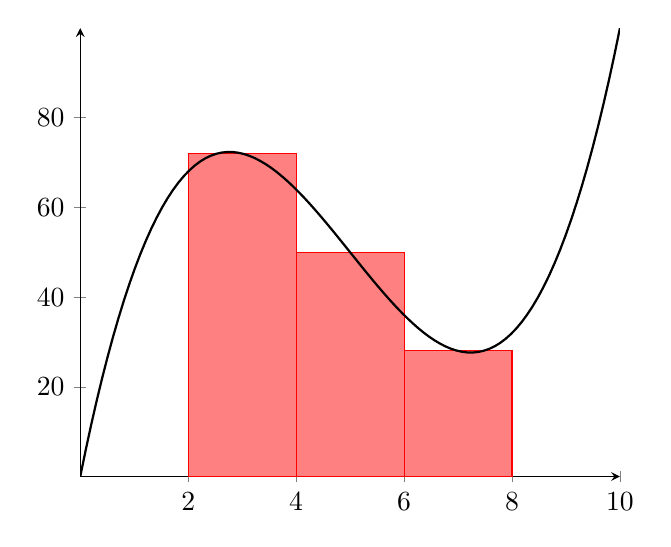
\begin{tikzpicture}[/pgf/declare function={f=-15*(x-5)+(x-5)^3+50;}]
    \begin{axis}[
        domain=0:10,
        samples=100,
        axis lines=middle
    ]
    \addplot [
        red,
        fill=red!50,
        integral=2:8
    ] {f};
    \addplot [thick] {f};
    \end{axis}
  \end{tikzpicture}
\end{align}
\begin{align*}
  \text{Esempio di somma di Riemann di una funzione $f:[2,8]\to\mathbb{R}$ con n=3:}
\end{align*}
\thm{Integrabilita' delle funzioni continue}{
  Sia $f:[a,b]\to\mathbb{R}$ continua. Sia $(S_n)$ la successione delle somme di Riemann, allora:
  \[
    \lim_{n\to +\infty} S_n = l \in \mathbb{R}
  \]
  E non dipende da quale $\epsilon_n$ scegliamo per ogni segmento.
}
\nt{
  In realta', una funzione e' Riemann integrabile anche se non e' continua, basta che l'insieme di punti di discontinuita' sia al massimo numerabile.
}
Possiamo esprimere il limite infinito di questa somma di rettangoli infinitesimi con il simbolo di \textbf{integrale}:
\dfn{Integrale}{
  \[
    \int_{a}^{b} f(x)dx = \lim_{n\to+\infty} S_n
  \]
  La x e' una variabile \textbf{muta}. 
}
\nt{
\begin{itemize}
  \item Se $\forall x \in [a,b]. f(x) \geq 0$, allora $\int_a^b f$ = Area del sottografico.
  \item $\int_a^a f = 0$ (poiche $\forall n \in \mathbb{N}. S_n = 0$)
  \item $ f(x) = k (\text{funzione costante}) \implies \int_{a}^{b}f = (b-a)k (\text{Area del rettangolo}) $
\end{itemize}
}
\subsection{Proprieta' dell'integrale}
\subsubsection{Linearita'}
Se abbiamo due funzioni f, g continue su [a,b], $A, \mu \in \mathbb{R}$
\[
  \int^b_a (Af(x)+\mu g(x))dx = A\int^b_a f(x)dx + \mu\int^b_a g(x)dx
\]
\subsubsection{Additivita}
Data $f:[a,b]\to\mathbb{R}$ continua, dato $c \in [a,b]$, vale: \label{HA}
\[
\int^b_a f = \int^c_a f + \int^b_c f
\]
\nt{
Convenzione su integrali con estremi "rovesciati":\\
Dato $f:[a,b]\to\mathbb{R}$
\[
\int^b_a f = -\int^a_b f
\]
}
In questo modo possiamo generalizzare la proprieta' addittiva togliendo dall' ipotesi la restrizione sul valore di c.
\subsubsection{Monotonia}
Se $f:[a,b]\to\mathbb{R}$ e $\forall x \in [a,b]. f(x) \geq 0$, allora:
\[
\int^b_a f \geq 0 
\]
\subsection{Media Integrale}

\textbf{Premessa 1}\\
\thm{Valori intermedi}{
  Sia $f:[a,b]\to\mathbb{R}$ continua, $x_1, x_2, \in [a,b]. f(x_1) \leq f(x_2)$, allora:
  \[
    \forall y \in [f(x_1), f(x_2)].\exists c \in [x1, x2].f(c)=y
  \]
  
}
\textbf{Premessa 2}\\
\thm{Weierstrass}{
  Sia $f:[a,b]\to\mathbb{R}$ continua:
  \[
    \exists x_1, x_2 \in [a,b].\forall x \in [a,b]. f(x_1) \leq f(x) \leq f(x_2)
  \]
  Quindi una funzione continua su dominio chiuso e limitato ha massimo e minimo assoluti.
}
\begin{figure}[h!]
    \centering
    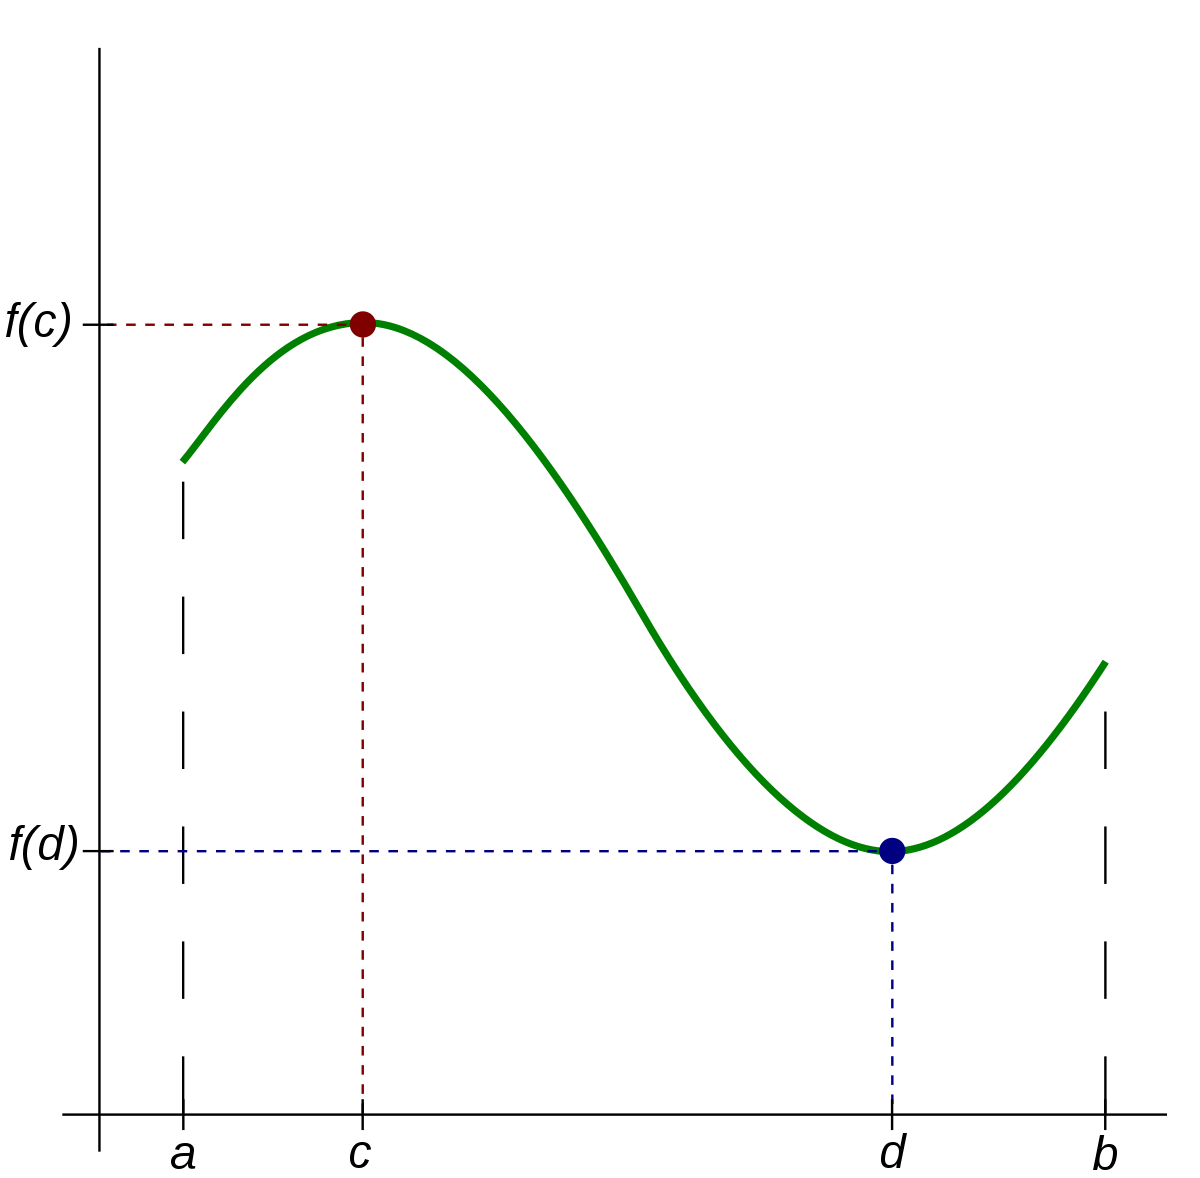
\includegraphics[width=50mm]{img/1200px-Extreme_Value_Theorem.svg.png}
    \caption{Esempio di Weierstrass}
  \end{figure}

\thm{Media integrale}{
  Sia $f:[a,b]\to\mathbb{R}$ continua, allora:
  \[
    \exists c \in [a,b]. \frac{1}{b-a}\int^b_a f(x)dx = f(c)
  \]      
}

\begin{figure}[h!]
  \centering
  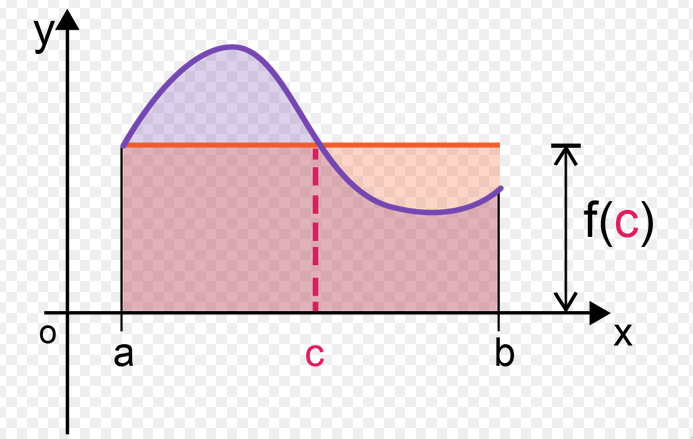
\includegraphics[width=100mm]{img/2024-02-23-16-46-38.png}
\end{figure}

Quindi esiste un punto c in [a,b] t.c. il rettangolo che ha come base b-a e come altezza f(c) ha la stessa area dell'integrale di f da a a b.\\

\pf{Dimostrazione della media integrale}{
  Sia f continua su [a,b]. Per Weierstrass abbiamo che $\exists x_1, x_2 \in [a,b].\forall x \in [a,b].f(x_1) \leq f(x) \leq f(x_2)$. Per la proprieta' di monotonia risulta $\int^b_a f(x_1)dx \leq \int^b_a f(x)dx \leq \int^b_a f(x_2)dx$, ovvero $f(x_1) \leq \frac{1}{b-a}\int^b_a f(x)dx \leq f(x_2)$. Quindi per il teorema dei valori intermedi $\exists c \in [a,b].f(c)=\frac{1}{b-a}\int^b_a f(x)dx$.
}

\nt{
  La continuita' di f e' \textbf{necessaria}. Ex:
  \[
    f:[-1,1] \to \mathbb{R}, f(x) = x \implies \frac{1}{2} \int_{-1}^{1}xdx = 0 = f(0) (c=0)
  \]
 \begin{align*} 
    \begin{tikzpicture}
      \draw[->] (-1.5,0)--(1.5,0) node[below] {$ x $};
      \draw[->] (0,-1.5)--(0,1.5) node[left] {$ y $};
      \draw[domain=-1:1] plot (\x, \x);
      \draw[dashed] (1,0)--(1,1) (0.7, 0.3) node{$ A_1 $};
      \draw[dashed] (-1,0)--(-1,-1) (-0.7, -0.3) node{$ A_2 $};
      \draw (1.5, 1.5) node{$ A_1 = -A_2 $};
    \end{tikzpicture}
 \end{align*}
  Se considerassi $ g:[-1,1] \to \mathbb{R}$
  \[
    g(x) = \begin{cases}
    x & x \neq 0\\
    2 & x = 0
    \end{cases}
  \]
  Si dimostra che g e' intagarbile, e che vale
  \[
    \int_{-1}^{1}g(x)dx = 0
  \]
  Pero' non esiste $ c \in [-1,1] $ tale che g(c) = 0, quindi non soddisfa la media integrale.
}

\section{Primitive di una funzione}
\dfn{Primitiva di f}{
  Sia $ f: A \to \mathbb{R}, A \subseteq \mathbb{R} $\\
  Una funzione $ F: A \to \mathbb{R} $ derivabile si dice primitiva di f su A se vale
  \[
    \forall x \in A. F'(x) = f(x)
  \]
}
\ex{Primitiva}{
  $ f:\mathbb{R}\to \mathbb{R} $, $f(x) = \cos x \implies F(x) = sin x$ e' una primitiva di f su $ \mathbb{R} $. Infatti $\forall x. \frac{d}{dx}sinx = cosx $
}
\nt{
  $ \forall k \in \mathbb{R}\text{, la funzione }G(x) = sin(x)+k $ e' anchessa primitiva di $ f $. Quindi se $ F $ e' primitiva di $ f $ su A allora ci sono infinite primitive di $ f $ su A (una per ogni $ k \in \mathbb{R} $).\\
}
Possiamo essere sicuri che queste sono tutte le possibili primitive?
\mprop{Caratterizzazione delle primitive di una funzione su un intervallo}{
  Sia $ f:]a,b[\to\mathbb{R}$. Siano $F:]a,b[\to\mathbb{R}\text{ e }G:]a,b[\to\mathbb{R}$ due primitive di $ f $ su $ ]a,b[ $.\\
  Allora $ \exists k \in \mathbb{R} $ tale che:
  \[
    \forall x \in ]a,b[. G(x)=F(x)+k
  \]
  Ovvero $ F $ e $ G $ "differiscono per una costante".
}
\pf{Dimostrazione}{
  Considero $ H:]a,b[\to\mathbb{R}, H(x)=G(x)-F(x) $. Sappiamo che F'(x)=f(x) e G'(x)=f(x) (def. primitiva).
  $ \frac{d}{dx}H(x) = \frac{d}{dx}G(x)-\frac{d}{dx}F(x) = f(x)-f(x) = 0 $. Dunque $ H $ ha derivata nulla su $ ]a,b[ $, quindi (per coroll. Lagrange) $ H $ e' costante.
}

\section{Funzioni integrali}
D'ora in poi $ A = ]a,b[ $.
\dfn{Funzione Integrale}{
  Sia $ f:A\to\mathbb{R} $ continua.\\
  Sia $ c\in A $. Introduco $ I_c:A\to\mathbb{R} $:
  \[
    I_c(x) = \int_{c}^{x}f(t)dt
  \]
  Nota: $ I_c $ e' ben definita essendo f continua.
}
\nt{
  \begin{enumerate}
    \item $ f:A\to\mathbb{R}, c\in A, I_c(x) = \int_{c}^{x}f \implies I_c(c)=\int_{c}^{c}f(t)dt = 0 $.
    \item Dati $ c,c' \in A, f:A\to\mathbb{R} \implies I_c(x)-I_{c'}(x) $ = costante. Infatti:
      \[
        I_c(x) - I_{c'}(x) = \int_{c}^{x}f(t)dt - \int_{c'}^{x}f(t)dt = \int_{c}^{x}f(t)dt + \int_{x}^{c'}f(t)dt = \int_{c}^{c'}f(t)dt = k
      \]
  \end{enumerate}
}
\subsection{Teoremi fondamentali del calcolo integrale}
\thm{Fondamentale del calcolo sulla derivata della funzione integrale}{
  Sia $ f:A\to\mathbb{R} $ continua, $ c \in A $. Sia $ I_c $ la funzione integrale, allora:
  \[
    I_c \text{ e' derivabile in ogni punto } x \in A \text{ e } I_c'(x) = f(x)
  \]
  Cioe' $ \frac{d}{dx}\int_{c}^{x}f(t)dt = f(x), \forall x \in A $, quindi $ I_c $ e' \textbf{primitiva} di $ f(x) $.
}
Una possibile interpretazione di questo teorema e' quello della derivata dell'area sottesa che e' uguale alla funzione stessa, ovvero:
\[
  \forall x. f(x) \geq 0 \implies \frac{d}{dx} \text{Area} = f(x)
\]
$ A = ]-2,2[, f(x)=\frac{x^2}{5} + 1 $:\\
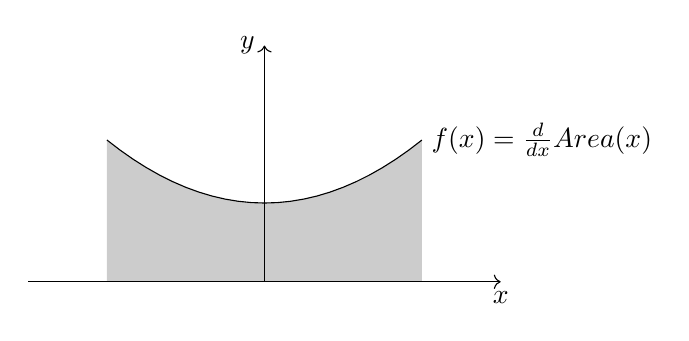
\begin{tikzpicture}
  \fill[gray!40, domain=-2:2, variable=\x]
   (-2,0)
   -- plot (\x, \x*\x/5 + 1)    
   -- (2,0)
   -- cycle;
   \draw[domain=-2:2] plot (\x, {(\x*\x/5 + 1)}) node[right]{$ f(x) = \frac{d}{dx}Area(x) $};

   \draw[->] (-3,0)--(3,0) node[below]{$ x $};
   \draw[->] (0,0)--(0,3) node[left]{$ y $};
\end{tikzpicture}
\begin{tikzpicture}

  \draw[domain=-2:2] plot (\x, {\x/2*(1+(\x*\x/15)) + 19/15}) node[right]{$ Area(x) = \int_{-2}^{x}f(x)dx $};
   \draw[->] (-3,0)--(3,0) node[below]{$ x $};
   \draw[->] (0,0)--(0,3) node[left]{$ y $};
\end{tikzpicture}
\nt{
  Il teorema assicura che ogni funzione $ f:A\to\mathbb{R} $ continua ammette primitive.
}
\pf{Dimostrazione}{
  $ f:A\to\mathbb{R}, c\in A, I_c:A\to\mathbb{R} $. Devo calcolare la derivata di $ I_c $. Calcolo $ \lim_{h\to 0^+}\frac{I_c(x+h)-I_c(x)}{h} $, che equivale a $ \lim_{h\to 0^+}\frac{1}{h} \int_{x}^{x+h}f(t)dt $. Per teo. media integrale sappiamo che $ \exists c \in [x,x+h]. f(c) = \frac{1}{h}\int_{x}^{x+h}f(t)dt $, quindi possiamo riscrivere la formula come $ \lim_{h\to 0^+}f(c_h) $. Dato che $ h \to 0^+ $ e $ x \leq c \leq x+h $, per il teo. dei carabinieri $ c=x $, quindi (grazie alla continuita' di $ f $), $ \lim_{h\to 0+}f(c_h) = f(x) $.
}

\thm{Fondamentale del calcolo per integrali definiti}{
  Sia $ f:A\to\mathbb{R} $ continua su A. Sia $ F:A\to\mathbb{R} $ primitiva di f su A. Dati $ a,b\in A $, vale:
  \[
    \int_{a}^{b}f(x)dx = [F(b) - F(a)] = [F(x)]_a^b
  \]
}
\pf{Dimostrazione}{
  Sia $ c\in A $, $ I_c:A\to \mathbb{R} $ la funzione integrale ($ I_c(x) = \int_{c}^{x}f $). Per il teo. fond. del calc. sulla derivata di $ I_c $, $ I_c $ e' una primitiva di f su A. Per le proprieta' delle primitive, $ \exists k \in \mathbb{R}.\forall x \in A.F(x)=I_c(x)+k $. 
  \[
    F(b)-F(a)=(I_c(b)+k)-(I_c(a)+k)=I_c(b)-I_c(a)=\int_{c}^{b}f-\int_{c}^{a}f=\int_{a}^{c}f+\int_{c}^{b}f=\int_{a}^{b}f
  \]
}

\subsection{Integrazione per parti}
Si parte dalla regola del prodotto delle derivate ($ \frac{d}{dx}f(x)\cdot g(x) = f'(x)g(x)+f(x)g'(x) $) per trovare una regola di integrazione.
\thm{Integrazione per parti}{
  Dati $ f,g:A\to\mathbb{R} $, A intervallo aperto e sia $ F $ primitiva di $ f $ su $ A $ con $g$ derivabile e $ f,F,g' $ continue:
  \[
    \int_{a}^{b}\frac{d}{dx}(F(x)g(x))dx = \int_{a}^{b}f(x)g(x)dx + \int_{a}^{b}F(x)g'(x)dx
  \]
  Quindi usando il teorema fondamentale:
  \[
    [F(x)g(x)]_a^b = \int_{a}^{b}f(x)g(x)dx + \int_{a}^{b}F(x)g'(x)dx
  \]
  \[
    \int_{a}^{b}f(x)g(x)dx = [F(x)g(x)]_a^b - \int_{a}^{b}F(x)g'(x)dx
  \]
}

\subsection{Cambio di variabile}
\thm{Formula del cambio di variabile}{ \label{cambVar}
  Date $ h:I\to A $, $ f:A\to\mathbb{R} $, $ I,A \subseteq \mathbb{R} $ e $ \exists(f\circ h): I\to\mathbb{R}.(f\circ h)(t)=f(h(t)) $. $ f $ continua, $ h $ derivabile e $ h' $ continua. Presi $ \alpha,\beta\in I $, vale:
  \[
    \int_{h(\alpha)}^{h(\beta)} f(x)dx = \int_{\alpha}^{\beta}f(h(t))h'(t)dt
  \]
  Questa e' la versione generalizzata del teo. fond. del calcolo
}
\pf{Dimostrazione}{
  Date due funzioni $G,H: I\to\mathbb{R}. G(z) = \int_{\alpha}^{z}f(h(t))h'(t)dt, H(z) = \int_{h(\alpha)}^{h(z)}f(x)dx $, dobbiamo dimostrare che $ G(z) = H(z) $. Ci riduciamo a dimostrare che:
  \begin{enumerate}
    \item $ G(\alpha) = H(\alpha) $: ovvio perche' integrali su intervallo degenere ($ G(\alpha)=H(\alpha)=0 $)
    \item $ \forall z \in I.G'(z)=H'(z) $:
      \begin{itemize}
        \item $ G'(z) = \frac{d}{dz}\int_{\alpha}^{z}f(h(t))h'(t)dt = f(h(z))h'(z) $
        \item $ H'(z) = \frac{d}{dz}\int_{h(\alpha)}^{h(z)}f(x)dx = f(h(z))h'(z) $ (generalizzazione del teorema fondamentale del calcolo)
      \end{itemize}
  \end{enumerate}
}
\nt{
  \begin{enumerate}
    \item t integrata in $ \alpha,\beta $, allora x sara' integrata in $ h(\alpha),h(\beta) $.
    \item $ dx $ si e' trasformato in $ h'(t)dt $ ($ \frac{d}{dt}h(t) = h'(t) \implies dh(t) = h'(t)dt $)
  \end{enumerate}
}

\section{Integrali generalizzati (impropri)}
\dfn{Integrali generalizzati su intervalli illimitati}{
  Sia $ f: [a, +\infty[\to\mathbb{R} $. Si dice che l'integrale generalizzato $ \int_{a}^{+\infty} f(x)dx $ e' \textbf{convergente} se e' finito il limite $ \lim_{r\to+\infty}\int_{a}^{r}f(x)dx \coloneq \int_{a}^{+\infty}f(x)dx $. Altrimenti se il limite diverge o oscilla e' detto \textbf{divergente} (o oscillante).\\
  La definizione e' analoga per $ \int_{-\infty}^{a}f(x)dx $.
}

\dfn{Integrali generalizzati su intervalli limitati}{
  Sia $ f: ]a, b]\to\mathbb{R} $. Si dice che l'integrale $ \int_{a}^{b}f(x)dx $ e' \textbf{convergente} se il limite $ \lim_{r\to a^+}\int_{r}^{b}f(x)dx $ e' finito. Altrimenti se il limite diverge o oscilla e' detto \textbf{divergente} (o oscillante).\\
  La definizione e' analoga per $ f: [a, b[\to\mathbb{R} $.
}

\chapter{Spazio euclideo $\mathbb{R}^n$}
(Spazio \textbf{euclideo} = c'e' il prodotto scalare)\\
$ \mathbb{R}^n = \{x=(x_1,x_2,...,x_n)|\forall j\in \{1,2,...,n\}.x_j \in \mathbb{R} \} = \mathbb{R} \times \mathbb{R} \times ... \mathbb{R} $ (n volte).
\begin{itemize}
\item $ n=1 $ retta reale
\item $ n=2 $ piano cartesiano
\item $ n=3 $ spazio ordinario
\end{itemize}
\section{Operazioni su $ \mathbb{R}^n $}
\begin{itemize}
  \item Somma di vettori: $ x=(x_1,...,x_n), y=(y_1,...,y_n) $. Definiamo $ x+y=(x_1+y_1,...,x_n+y_n) \in \mathbb{R}^n $
  \item Prodotto di $ x\in\mathbb{R}^n $ per uno scalare $ \lambda \in \mathbb{R} $. Dato $ x=(x_1,...,x_n), \lambda \in \mathbb{R} $, definiamo $ \lambda x= (\lambda x_1, ..., \lambda x_n) $.
\end{itemize}

\dfn{Prodotto scalare}{
  Dati $ x,y \in \mathbb{R}_n $, definiamo il prodotto scalare $ <x,y> = \sum_{k=1}^{n}x_ky_k=x_1y_1+...+x_ny_n \in \mathbb{R}^n  $.\\
  Notazione alternativa: $ <x,y> = x \cdot y $.
}
\nt{
  Il prodotto scalare non da' un nuovo vettore, ma solo un valore scalare!
}
\subsection{Proprieta' del prodotto scalare (euclideo)}
\begin{itemize}
  \item $ \forall x,y \in \mathbb{R}^n. <x,y> = <y,x> $ (simmetria)
  \item $ \forall x,y,z \in \mathbb{R}^n, \lambda, \mu \in \mathbb{R}. <\lambda x+\mu y, z> = \lambda<x,z> + \mu<y,z> $ (linearita' nel primo argomento)\\
    Per simmetria vale $ <z, \lambda x + \mu y> = \lambda<z,x> + \mu<z,y> $ (linearita' nel secondo argomento)
  \item $ \forall x \in \mathbb{R}^n. <x,x> \geq 0 $, inoltre $ <x,x> = 0 \iff x = (0,0,...,0) = \underline{0} $ (vettore nullo). 
\end{itemize}

\section{Ortogonalita'}
\dfn{Vettori ortogonali}{
  Due vettori $ x,y \in \mathbb{R}^n $ si dicono \textbf{ortogonali} se vale:
  \[
  <x,y> = 0
  \]
}

\section{Norma euclidea}
Sinonimi: modulo, lunghezza
\dfn{}{
  Dato $ x \in \mathbb{R}^n $, allora 
  \[
  \lVert x \rVert = \sqrt{<x,x>} \geq 0
  \]
  Rappresenta la "lunghezza" del vettore usando il teorema di Pittagora. \\
  Notazione alternativa: $ |x| $
}
\subsection{Proprieta' della norma}
\begin{itemize}
\item $ \forall x \in \mathbb{R}^n. \lVert \lambda x \rVert = |\lambda| \cdot \lVert x \rVert $
\item $ \forall x \in \mathbb{R}^n. \lVert x \rVert = 0 \iff x = 0 $
\item $ \forall x,y \in \mathbb{R}^n. |x+y| \leq |x|+|y| $ (Disuguaglianza triangolare)
\end{itemize}
\section{Vettore normalizzato}
\dfn{Normalizzato}{
  Dato $ x \neq 0 \in \mathbb{R}^n $, cerco $ r > 0 $ t.c.
  \[
  |rx|=1
  \]
  Visto che $ r>0 $, $ r|x|=1 $ quindi $ r = \frac{1}{|x|} $.\\
  Il vettore $ \frac{x}{|x|} $ ha norma 1 e si dice \textbf{normalizzato} di $ x \in \mathbb{R}^n\setminus \{\underline{0}\} $.\\
  $ \frac{x}{|x|} $ si dice \textbf{vettore unitario}.
}
\nt{
  Possiamo scrivere $ x = |x|\cdot \frac{x}{|x|} $ se $ x \neq 0 $.
}
\section{Coordinate polari}
In $ \mathbb{R}^2 $, ogni $ (x,y)\neq(0,0) $ si scrive nella forma $ |(x,y)|\cdot (\frac{x}{|(x,y)|}, \frac{y}{|(x,y)|}) $. L'insieme di coordinate $ \{(\frac{x}{|(x,y)|}, \frac{y}{|(x,y)|})|x,y\in\mathbb{R}\} $ forma una \textbf{circonferenza unitaria} (dato che il loro modulo e' sempre 1), quindi $ \exists \theta \in [0,2\pi[ $ tale che $ (cos\theta, sin\theta) = (\frac{x}{|(x,y)|}, \frac{y}{|(x,y)|}) $ ($ \theta $ si chiama \textbf{"argomento"} di $ (x,y) $). Ponendo $ r = |(x,y)| = \text{modulo} $, scriviamo:
\[ (x,y) = r(cos\theta, sin\theta) \]
dove $ r > 0 $ e $ \theta \in [0,2\pi[ $ si chiamano \textbf{coordinate polari} di (x,y).

\begin{figure}[h!]
    \centering
    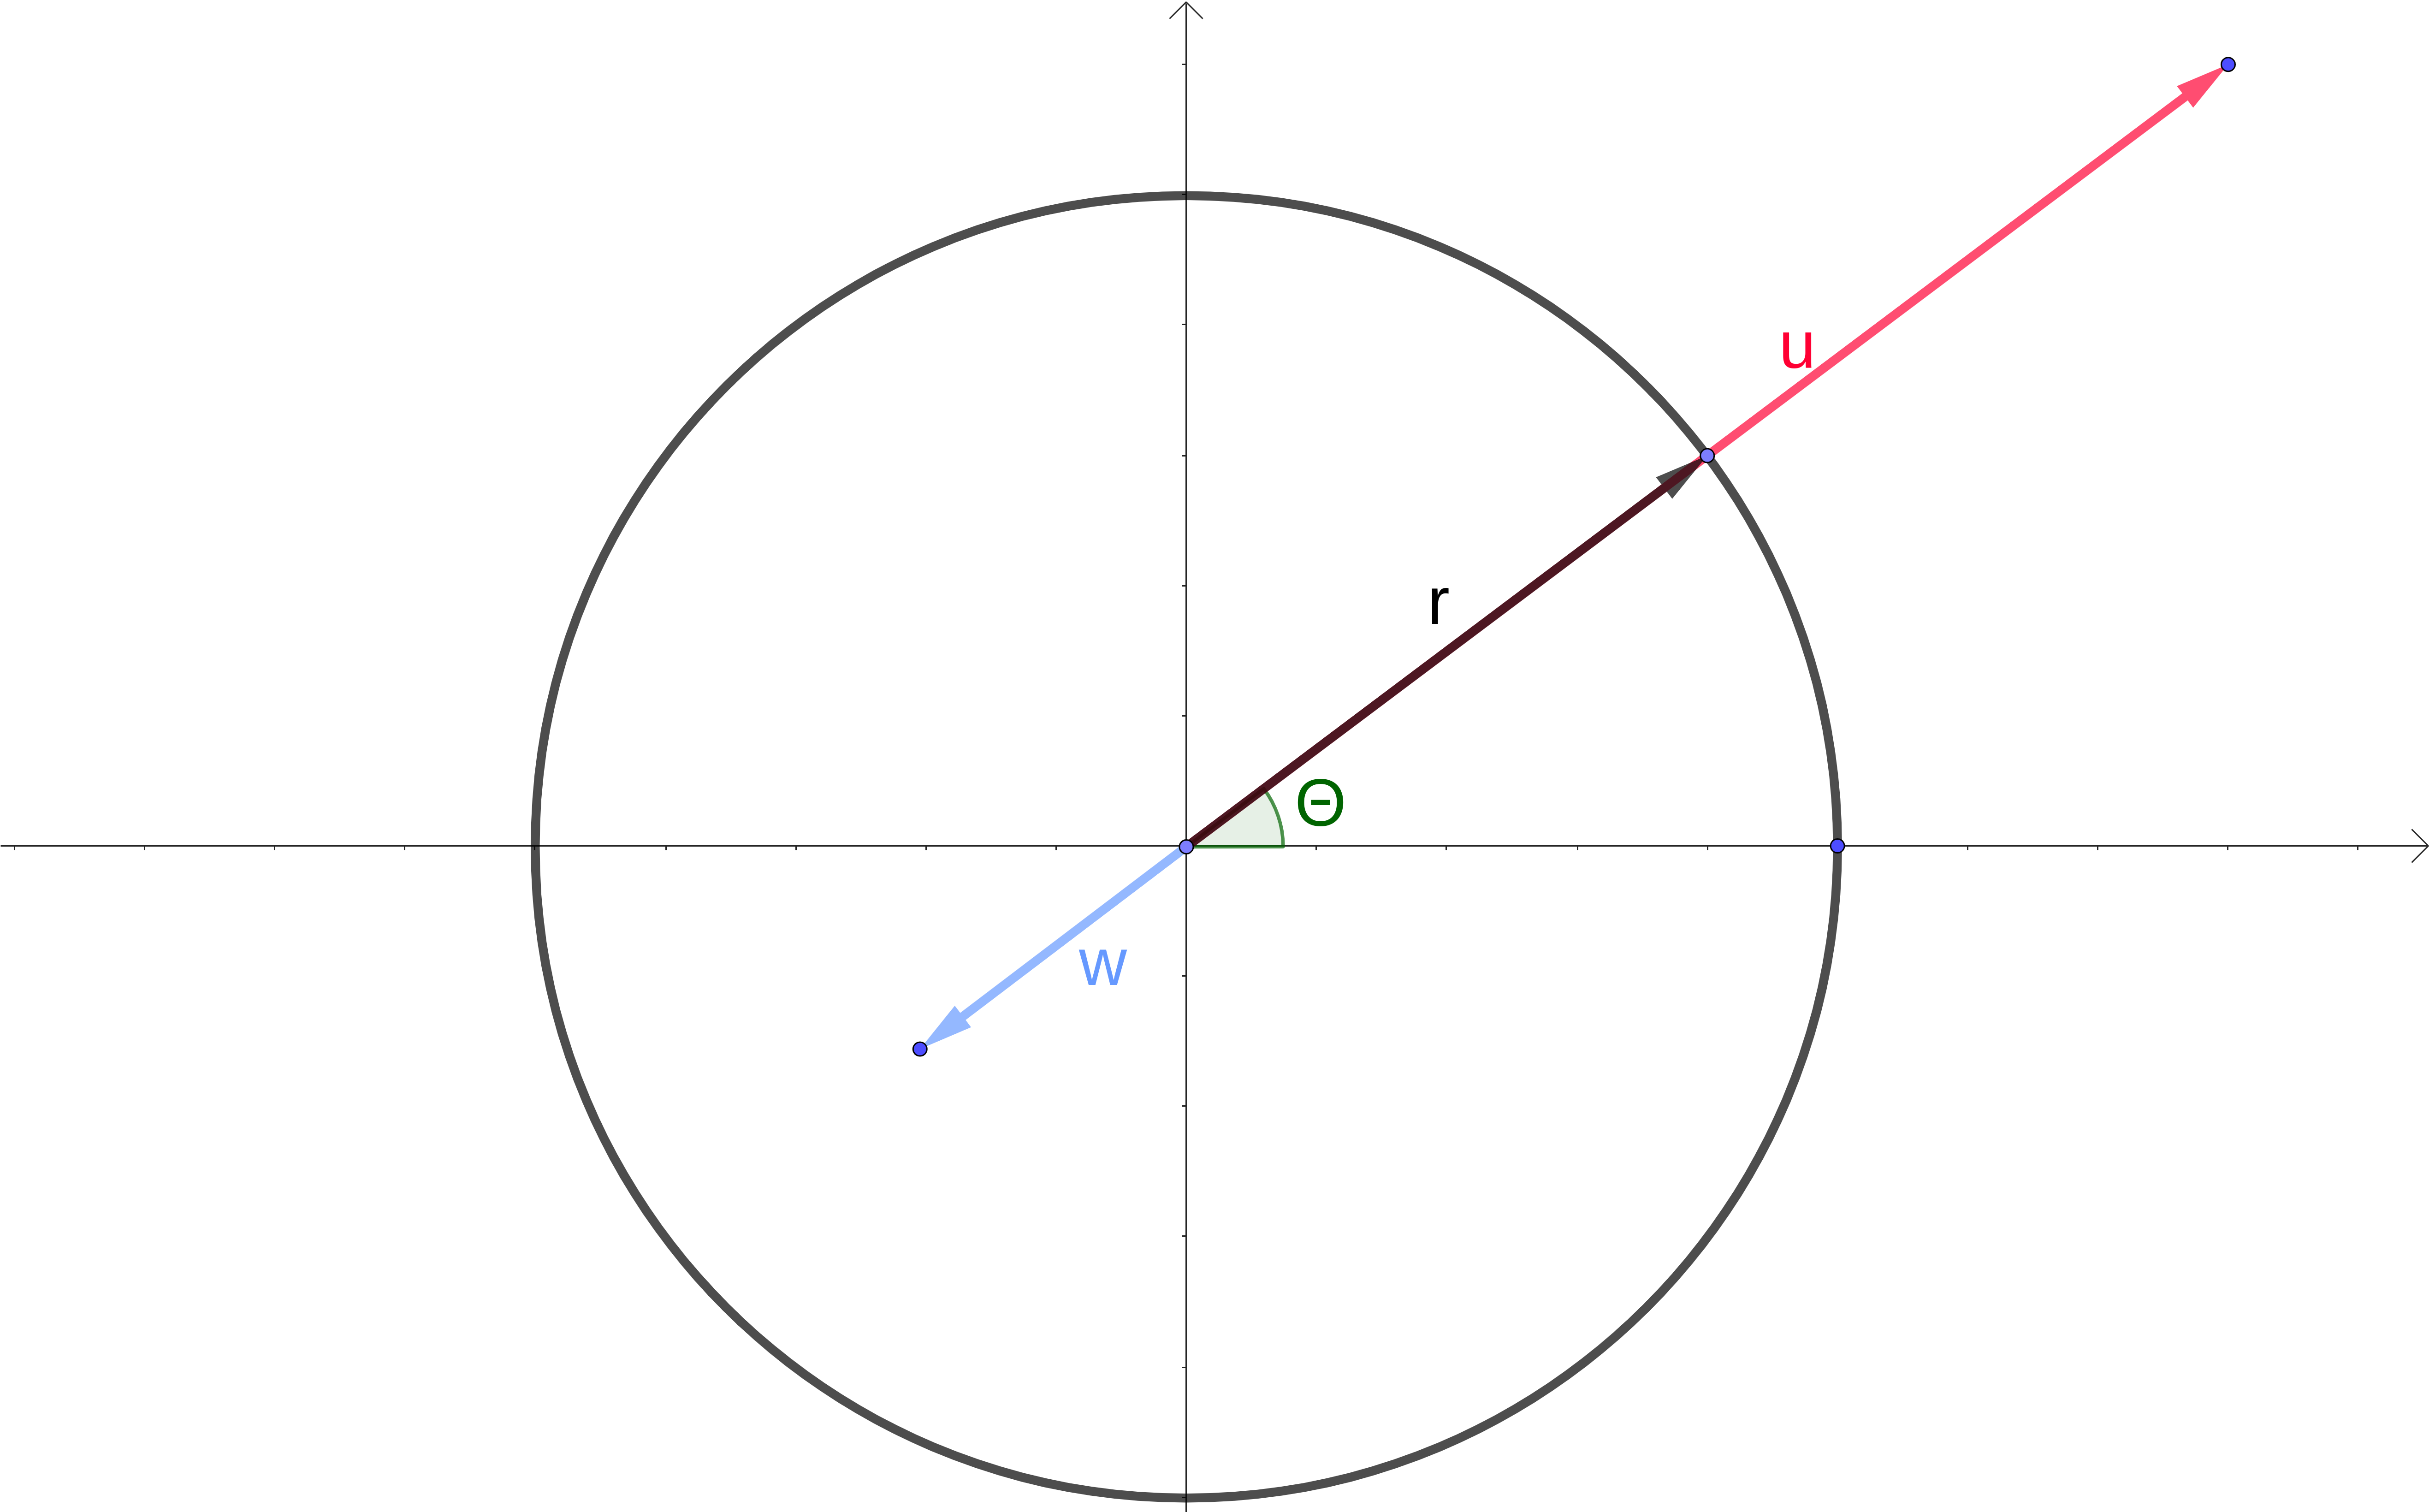
\includegraphics[width=0.3\textwidth]{img/2024-03-15-10-51-45.png}
    \begin{itemize}
    \item $ r =  $ vettore unitario
    \end{itemize}
\end{figure}


\subsection{Prodotto scalare in coordinate polari}
Considero due vettori $ (x,y) = (r cos\theta, r sin \theta) $ e $ (n,o) = (\rho cos \gamma, \rho sin\gamma) $. Il loro prodotto scalare $ <(x,y), (n,o)> $ diventa $ r\rho cos\theta cos\gamma + r\rho sin\theta sin\gamma $, che puo' essere riscritto come $ r\rho cos(\gamma - \theta) $, ovvero:
\[
  |(x,y)|\cdot|(n,o)|\cdot cos(\gamma - \theta)
\]
\mprop{Disuguaglianza di Cauchy-Schwarz}{ \label{cauchySchwarz}
  Dati $ x,y \in \mathbb{R}^n $, vale:
  \[
  |<x,y>| \leq \lVert x \rVert \cdot \lVert y \rVert
  \]
  L'uguaglianza vale solo se $ x $ e $ y $ sono linearmente dipendenti.
}
\nt{
  Vale in ogni $ \mathbb{R}^n \forall n \in \mathbb{N}$
}
\mprop{Quadrato di binomio}{
  \[
  |x+y|^2 = |x|^2 + |y|^2 + 2<x,y>
  \]
  Generalizzazione di Pitagora (In due dimensioni diventa il teorema di Carneau).
}
\mprop{Disuguaglianza Triangolare}{
  $ \forall x,y \in \mathbb{R}^n $ si ha che:
  \[
  |x+y| \leq |x| + |y|
  \]
}
\pf{}{
  Dimostriamo il quadrato della disuguaglianza per poter usare il quadrato di binomio:
  \[
    |x+y|^2 = |x|^2 + |y|^2 + 2<x,y> \leq |x|^2+|y|^2+2|<x,y>| \leq |x|^2+|y|^2+2|x||y| = (|x|+|y|)^2
  \]
  \[
    \implies |x+y|^2 \leq (|x|+|y|)^2
  \]
}
\begin{figure}[h!]
    \centering
    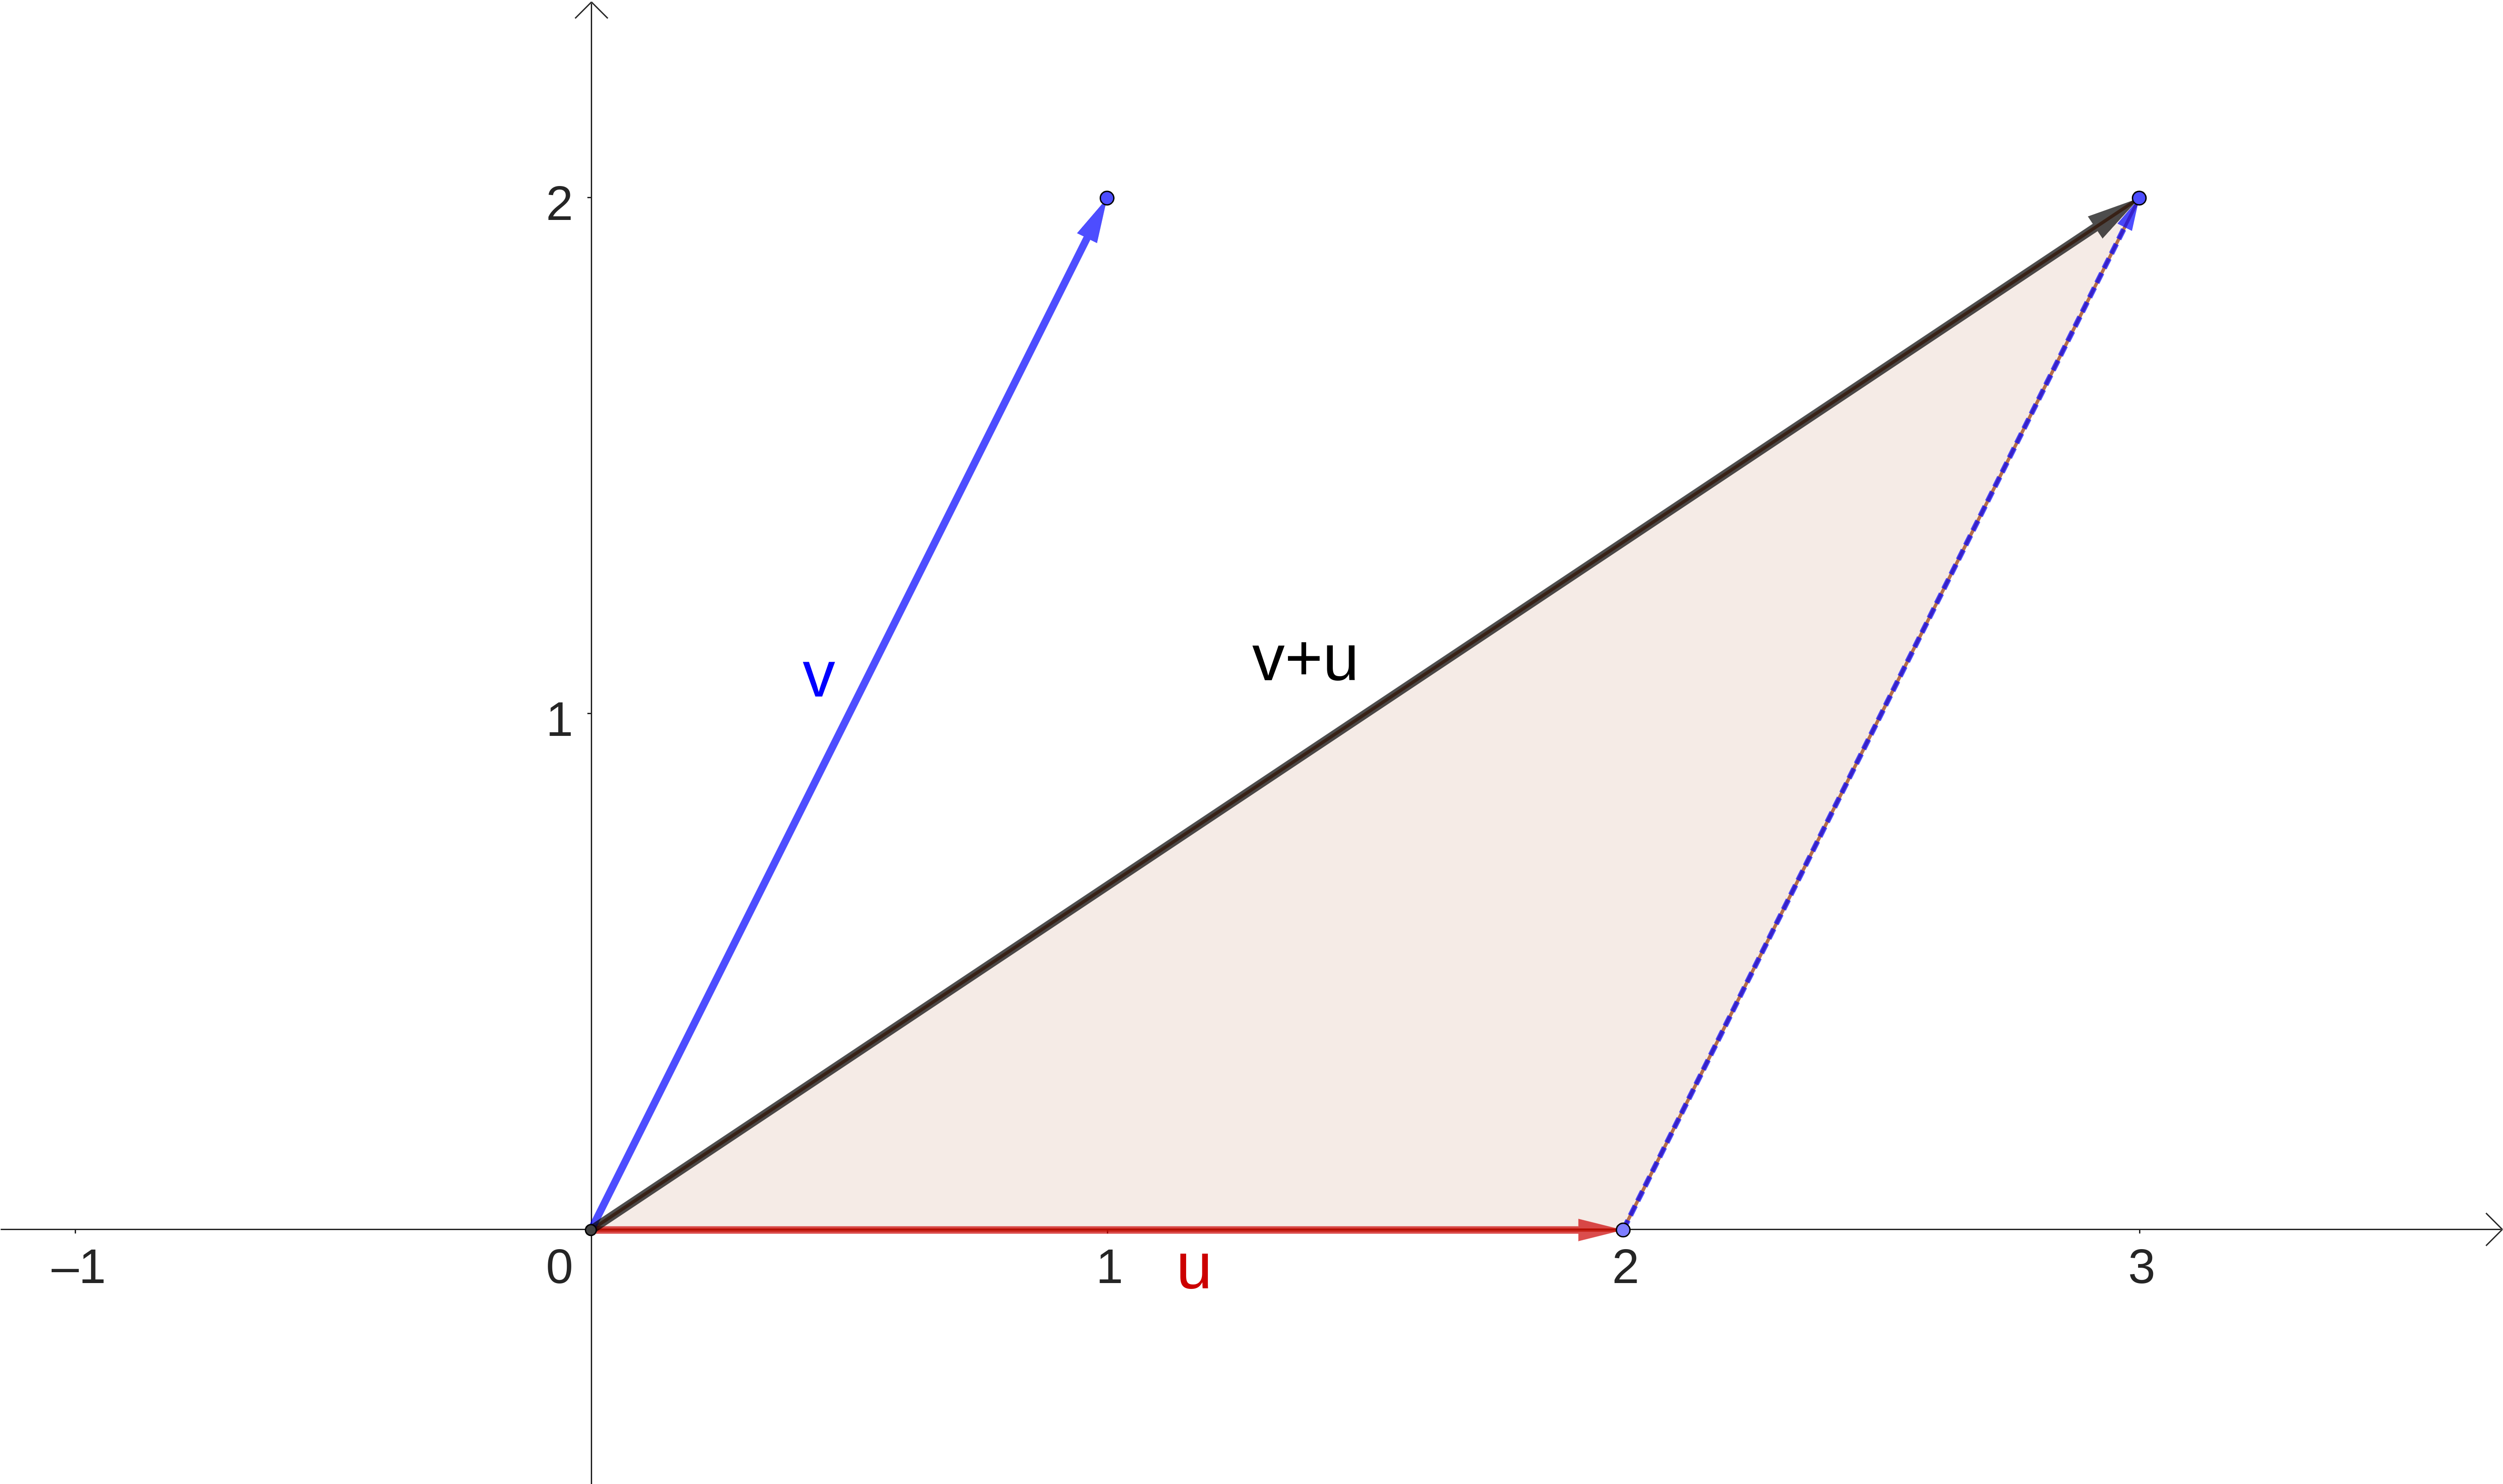
\includegraphics[width=0.6\textwidth]{img/2024-03-15-11-28-54.png}
\end{figure}


\section{Distanza tra punti}
\dfn{Distanza fra due punti}{
  Dati $ x,y \in \mathbb{R}^n $, la distanza fra $ x $ e $ y $ e' $ |x-y| $
}

\subsection{Punto di minima distanza da una retta}
Problema $ \mathbb{R}^n, v\neq 0, x \in \mathbb{R}^n $. Considero le linee $ l_v = \{tv|t\in\mathbb{R}\} $, cerco fra tutti i punti di $ l_v $ quello che ha minima distanza da $ x $. Devo minimizzare la funzione $ h:\mathbb{R}\to\mathbb{R}, h(t)=|x-tv| = \text{distanza fra x e tv} $, che (essendo non negativa), equivale a minimizzare la funzione alla seconda $ g(t) = |x-tv|^2 $. Usando il quadrato di binomio, otteniamo $ g(t) = |x|^2 + t^2|v|^2-2t \innerproduct{x}{v} $, ovvero una parabola con concavita' verso l'alto. Quindi il punto di minimo e' l'unico punto stazionario:
\[
  g'(t) = 2t|v|^2 -2 \innerproduct{x}{v} = 0 \iff t = \frac{\innerproduct{x}{v}}{|v|^2} = \overline{t}
\]
Quindi basta moltiplicare $ \overline{t} $ per $ v $ per trovare il punto di minima distanza:
\mprop{Punto di minima distanza da una retta}{
  Dati $ v \neq 0, x \in \mathbb{R}^n $ e la retta $ l_v = \{tv | t \in \mathbb{R}\} $, il punto $ \overline{t}v $ di minima distanza da $ x $ e':
  \[
  \overline{t}v = \frac{\innerproduct{x}{v}}{|v|^2}v
  \]
  E la distanza vale $ \sqrt{|x|^2 - \frac{\innerproduct{x}{v}^2}{|v|^2}} $.
}
Inoltre, come possiamo intuire, il vettore della minima distanza da $ l_v $ a $ x $ e' ortogonale a $ v $:
\mprop{Ortogonalita' distanza minima}{
  Dati $ v\neq 0 $ e $ x \in \mathbb{R}^n $, il punto di minima distanza $ \overline{t}v $ soddisfa:
  \[
  <x-\overline{t}v, v> = 0
  \]
  Quindi il vettore che parte dal punto di minima distanza e arriva al punto x e' perpendicolare alla retta $ l_v $.
}
\pf{Verifica}{
  (Basta svolgere i calcoli)
}

\section{Intorni}
Generalizziamo in $ \mathbb{R}^n $ il concetto di intorno di un punto e di insiemi aperti/chiusi, che ci saranno utili per definire derivate in $ n $ dimensioni:
\dfn{Intorno sferico di un punto}{
  Dato $ x \in \mathbb{R}^n $, $ r > 0 \in \mathbb{R} $, poniamo
  \[
    D(x,r) = \{y\in \mathbb{R}^n | |x-y| < r\}
  \]
  $ D(x,r) $ si dice disco di centro $ x $ e raggio $ r $.
}
\begin{center}
  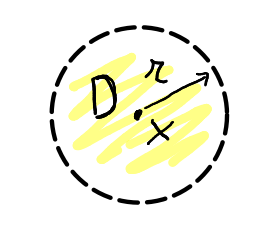
\includegraphics[width=0.2\textwidth]{img/2024-05-20-12-26-27.png}
\end{center}
\dfn{Insiemi aperti}{
  $ A \subseteq \mathbb{R}^n $ si dice aperto se:
  \[
    \forall x \in A. \exists \epsilon > 0.D(x,\epsilon) \subseteq A
  \]
}
\begin{center}
  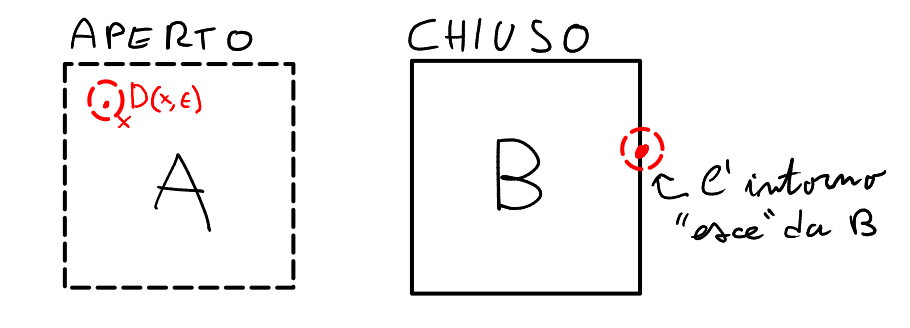
\includegraphics[width=0.5\textwidth]{img/2024-05-20-12-32-06.png}
\end{center}
\section{Successioni in $ \mathbb{R}^n $}
\dfn{Successione}{
  Una funzione $ x(k):\mathbb{N}\to\mathbb{R}^n $, indicata come $ x_k $, si chiama successione in $ n $ dimensioni ed e' un vettore di $ k $ successioni:
  \[
   x_k = (x_k^1, x_k^2, ..., x_k^n) \text{ con } k \in \mathbb{N} 
  \]
}
Come in una dimensione, una successione in $ n $ dimensioni e' convergente se:
\dfn{Successione convergente}{
   Sia $ x_k $ una successione in $ \mathbb{R}^n $ e $ x \in \mathbb{R}^n $. Si dice che $ x_k $ \textbf{converge} a $ x $ se $ \lim_{k\to +\infty}x_k = x $, ovvero se si verifica:
   \[
   \begin{cases}
   \lim_{k\to+\infty}x_k^1 = x^1 & \\
    \vdots & \\
    \lim_{k\to+\infty}x_k^n = x^n &
   \end{cases}
   \]
}
\mprop{}{
  Sia $ x_k $ una successione in $ \mathbb{R}^n $ e sia $ x \in \mathbb{R}^n $, si ha che:
  \[
  \lim_{k \to +\infty} x_k = x \iff \lim_{k\to+\infty} \norm{x_k - x} = 0
  \]
}
\nt{
  Per vedere se una successione in $ \mathbb{R}^n $ e' convergente, basta studiare la convergenza di una successione in $ \mathbb{R} $ ($ \norm{x_k-x}_k $)
}
\chapter{Funzioni a piu' variabili}
Dati $ A \subseteq \mathbb{R}^n, B \subseteq \mathbb{R}^q $, consideriamo funzioni $ f:A\to B $ (A = dominio, B = codominio).

Casi modello:
\begin{itemize}
  \item $ f:\mathbb{R}^n\to\mathbb{R} $ (funzioni scalari)
  \item $ f:\mathbb{R}\to\mathbb{R}^q $ (cammini in $ \mathbb{R}^q $)
\end{itemize}

\section{Insiemi di livello}
\dfn{}{
  $ A \subseteq \mathbb{R}^n, f:A\to\mathbb{R}, b \in \mathbb{R} $. L'insieme di livello $ b $ di $ f $ e':
  \[
    L_b = \{x \in A | f(x) = b \} = f^{-1}(b)
  \]
}
Se cammino lungo l'insieme di livello, la funzione corrispondente non cambia
\section{Continuita'}
\dfn{Funzioni continue}{
  $ A \subseteq \mathbb{R}^n, f:A\to\mathbb{R}, k \in A $. Si dice che $ f $ e' continua in $ k \in A $ se $ \forall (x_n)_{n\in\mathbb{N}} \in \mathbb{R}^n $ vale:
  \[
  \begin{cases}
  \forall n \in \mathbb{N}.x_n \in A & \\
    x_n \xlongrightarrow{n\to+\infty} k & 
  \end{cases} \implies f(x_n)\xlongrightarrow{n\to+\infty} f(k)
  \]
}
\mprop{}{
  Sia $ A \subseteq \mathbb{R}^n, f:A\to\mathbb{R}, k\in A $. Allora $ f $ e' continua in $ k $ se:
  \[
  \forall \epsilon > 0\exists\delta>0.\forall x \in A:|x-k|<\delta \implies |f(x)-f(k)|<\epsilon
  \]
  Ovvero, $ \lim_{x\to k}f(x) = f(k) $.
}

\section{Derivata parziale}
\dfn{Derivata parziale}{
  Data $ f:A\to \mathbb{R}, A \subseteq \mathbb{R}^2 $. Dati $ (\overline{x},\overline{y}) \in A $ $ f $ si dice derivabile parzialmente rispetto a $ \overline{x} $ se:
  \[
    \exists \lim_{h\to 0}\frac{f(\overline{x}+h,\overline{y})-f(\overline{x},\overline{y})}{h} = \frac{\partial f}{\partial x}(\overline{x}, \overline{y})
  \]
  In modo analogo per $ \frac{\partial f}{\partial y}(\overline{x}, \overline{y}) $.
}
\dfn{Gradiente}{
  Se $ f:\mathbb{R}^2\to\mathbb{R} $ ammette derivate parziali $ \forall(\overline{x}, \overline{y}) \in \mathbb{R}^2 $, definiamo il \textbf{gradiente di f} come:
  \[
    \nabla f(x,y) = (\frac{\partial f}{\partial x}(x,y), \frac{\partial f}{\partial y}(x,y))  
  \]
  $ \nabla f: \mathbb{R}^2\to\mathbb{R}^2 $ (funzione vettoriale)
}
\nt{
  $ f:\mathbb{R}^2\to\mathbb{R} $, $ (\overline{x}, \overline{y}) $ fissato:
  \[
    \partial_xf(\overline{x}, \overline{y}) = \lim_{h\to 0}\frac{f(\overline{x}+h,\overline{y})-f(\overline{x}, \overline{y})}{h} = \lim_{x\to \overline{x}}\frac{f(x, \overline{y})-f(\overline{x}, \overline{y})}{x-\overline{x}}
  \]
  Introduco una funzione $ g:\mathbb{R}\to\mathbb{R} $, $ g(x) = f(x,\overline{y}) $, in modo che, facendo la normale derivata di $ g $:
  \[
    g'(\overline{x}) = \lim_{x \to \overline{x}}\frac{g(x) - g(\overline{x})}{x-\overline{x}} = \frac{\partial f}{\partial x}f(\overline{x}, \overline{y})
  \]
  Abbiamo quindi trasformato una derivata parziale in una derivata "normale" fissando tutti i parametri tranne uno. 
}
\begin{figure}[h!]
    \centering
    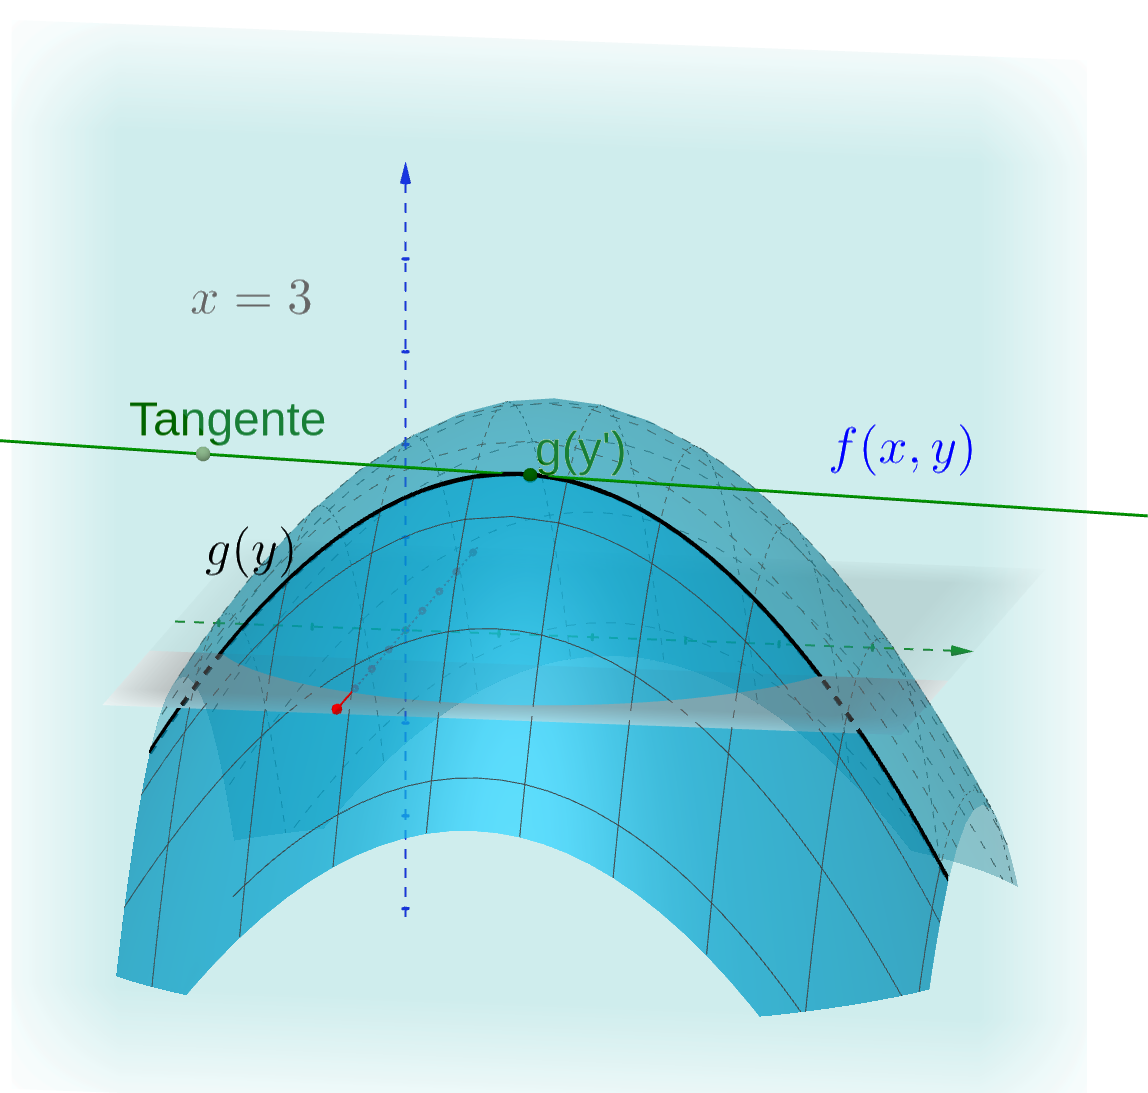
\includegraphics[width=0.5\textwidth]{img/2024-03-22-10-57-10.png}
\end{figure}

\subsection{Derivate parziali in $ \mathbb{R}^n $}
In $ \mathbb{R}^n $, data $ f:\mathbb{R}^2\to\mathbb{R} $ possiamo riscrivere la derivata parziale cosi:
\[
  \frac{\partial f}{\partial x}(\overline{x}, \overline{y}) = \lim_{t\to 0}\frac{f((\overline{x}, \overline{y}) +t(1,0))- f(\overline{x}, \overline{y})}{t}
\]
Possiamo usare quindi le basi canoniche $ (e_1 = (1,...,0),...,e_n(0,...,1)) $ per indicare per quale dei valori del vettore passato come parametro vogliamo derivare.
\dfn{}{
  $ f:\mathbb{R}^n\to\mathbb{R} $, $ x=(x_1,...,x_n), \overline{x} \in \mathbb{R}^n $. Per $ k = \{1,...,n\} $:
  \[
    \frac{\partial f}{\partial x_k}(\overline{x}) = \lim_{t\to 0}\frac{f(\overline{x} + te_k)-f(\overline{x})}{t}
  \]
}

\section{Derivabilita' e continuita'}
In $ \mathbb{R} $, se una funzione era derivabile in un punto allora era anche continua, pero' se in piu' variabili non e' cosi:(guardare es slide)

\section{Differenziabilita'}
In una dimensione, possiamo dire che:
\[
  \exists f'(\overline{x}) \in \mathbb{R} \iff f(\overline{x}+h) = f(\overline{x}) + f'(\overline{x})h + o(h)   
\]
Quindi una funzione e' derivabile in un punto sse vale lo sviluppo di Taylor. Infatti, se sostituiamo $ x $ a $ \overline{x} + h $, dove $ x\to \overline{x} $ otteniamo il polinomio di Taylor di primo grado nel punto $ \overline{x} $: $ f(x) = f(\overline{x}) + f'(\overline{x})(x - \overline{x}) + o(x - \overline{x}) $.\\
Come vedremo, questa prposizione non vale quando aumentiamo le dimensioni. Infatti, solo in una dimensione differenziabilita' e derivabilita' coincidono.
\subsection{o piccolo in piu' variabili}
\dfn{o piccolo}{
  Dati $ A \subseteq \mathbb{R}^n, h \in A, g:A\to\mathbb{R} $, assumendo che $ 0 \in A $, si dice che $ g $ e' \textbf{o piccolo} di $ |h|^p $ (con $ p \geq 0 $) se:
  \begin{enumerate}
    \item $ g(0) = 0 $
    \item $ \forall \epsilon > 0. \exists \delta > 0.\forall h \neq 0. |h| < \delta. \frac{|g(h)|}{||h||^p} < \epsilon $
  \end{enumerate}
}
\ex{}{
  Verifica le seguenti uguaglianze:
  \begin{itemize}
    \item $ g(h,k) = h^2 + k^2 = o(|h+k|) $
      \[
      h^2 + k^2 = |(h,k)|^2
      \]
      Quindi:
      \[
      \frac{|(h,k)|^2}{|(h,k)|} = |(h,k)|
      \]
      Dobbiamo dimostrare che $ \forall \epsilon > 0.\exists \delta > 0. \forall 0 < |(h,k)| < \delta. |(h,k)| < \epsilon $, che possiamo fare mettendo $ \delta = \epsilon $ per ogni $ \epsilon > 0 $.
  \end{itemize}
}
Possiamo riscrivere questa definizione usando le successioni:
\[
  g(h) = o(|h|^p) \iff \forall (h_j)_{j\in\mathbb{N}}. \begin{cases}
  h_j \neq 0 & \forall j \in \mathbb{N}\\
    \lim_{j\to+\infty}(h_j) = 0 & 
  \end{cases} \implies \lim_{j\to +\infty}\frac{g(h_j)}{||h_j||^p} = 0
\]
\dfn{Differenziabilita' in due variabili}{
  $ (x,y),(h,x)\in\mathbb{R}^2 $. Sia $ f:\mathbb{R}^2\to\mathbb{R} $. Sia $ (\overline{x}, \overline{y})\in\mathbb{R}^n $. Si dice che $ f $ e' differenziabile in $ (\overline{x}, \overline{y}) $ se:
  \begin{enumerate}
    \item $ \exists \partial_xf(\overline{x}, \overline{y}), \partial_yf(\overline{x}, \overline{y}) $
    \item Vale lo sviluppo:
      \[
        f((\overline{x}, \overline{y})+(h,k)) = f(\overline{x}, \overline{y}) + <\nabla f(\overline{x}, \overline{y}), (h,k)> + o(|(h,k)|) = 
      \]
      \[
        f(\overline{x}, \overline{y}) + \partial_xf(\overline{x}, \overline{y})h + \partial_yf(\overline{x}, \overline{y})k + o(|(h,k)|)
      \]
      Per $ (h,k) \to (0,0) $
  \end{enumerate}
}

\section{Continuita' di una funzione differenziabile}
Sappiamo che l'esistenza delle derivate parziali non implica la continuita' della funzione. Mostreremo pero' che se sappiamo che una funzione e' differenziabile, allora sara' sicuramente continua.
\mprop{Differenziabilita' implica continuita'}{
  Data $ f:\mathbb{R}^2\to\mathbb{R} $, se $ f $ e' differenziabile in $ (\overline{x}, \overline{y}) \in \mathbb{R}^2 $, allora $ f $ e' continua in $ (\overline{x}, \overline{y}) $.
}
\pf{}{
  Verifichiamo che la proposizione valga. Per ipotesi, sappiamo che $ f $ e' differenziabile in $ (\overline{x}, \overline{y}) \in \mathbb{R}^2 $. Quindi $ f(\overline{x}+h, \overline{y}+k) = f(\overline{x}, \overline{y}) + \innerproduct{\nabla f(\overline{x}, \overline{y})}{(h,k)} + o(|h,k|) $ (TODO: capire perche' questa vale solo quando (h,k) tende a (0,0)). Dobbiamo dimostrare che $ f $ sia continua in $ (\overline{x}, \overline{y}) $, ovvero che (usando la definizione di continuita' per successioni): $ \forall (h_j, k_j): \mathbb{N} \to \mathbb{R}^2. (h_j, k_j) \xlongrightarrow{j\to +\infty}(0,0). \lim_{j\to +\infty} f(\overline{x}+h_j, \overline{y}+k_j) = f(\overline{x}, \overline{y}) $. Quindi usando la nostra ipotesi possiamo ridurci a dimostrare che $ \lim_{j \to +\infty} \innerproduct{\nabla f(\overline{x}, \overline{y})}{(h_j,k_j)} + o(|h_j,k_j|) = 0 $. Dato che $ (h_j, k_j) $ tende a $ (0,0) $ per $ j $ che tende a $ +\infty $, il prodotto scalare diventa nullo. Per quanto riguarda l'o-piccolo, possiamo usare la sua proprieta' per cui $ \lim_{j\to +\infty} \frac{o(|h_j, k_j|)}{|h_j, k_j|}  = 0 $ riscrivendolo come $ \frac{o(|h_j, k_j|)}{|h_j, k_j|}|h_j, k_j| $. Con $ j \to +\infty $ sia la frazione che il fattore moltiplicativo tendono a $ 0 $. 
}
\section{Condizioni sufficenti per la differenziabilita'}
\thm{}{
  Sia $ f:\mathbb{R}^2\to\mathbb{R} $. Assumo che esistano continue $ \partial_xf(\overline{x}, \overline{y}), \partial_yf(\overline{x}, \overline{y}) $ per ogni $ (\overline{x}, \overline{y}) \in \mathbb{R}^2 $, allora:
  \[
  f \text{ e' differenziabile in ogni punto di } \mathbb{R}^2
  \]
}
\nt{
  Questo teorema vale anche in $ \mathbb{R}^n $. Inoltre le funzioni elementari soddisfano sempre le ipotesi nel loro dominio, quindi sono differenziabili.
}
Per dimostrare questo teorema, ci serve prima una proposizione che equivale al teorema di Lagrange, pero' in piu' dimensioni. Usando le derivate parziali, ci riduciamo a due casi (uno dove ci si muove lungo $ x $, e uno lungo $ y $) dove ci riduciamo ad una funzione $ \mathbb{R}\to\mathbb{R} $ che sappiamo gia' dimostrare.
\mprop{Lagrange per derivate parziali}{
  Sia $ f:\mathbb{R}^2\to\mathbb{R} $ una funzione con derivate parziali $ \partial_xf, \partial_yf $ continue, $ \forall (\overline{x}, \overline{y}), (h,k) \in \mathbb{R}^2. \exists \delta,\overline{\delta} \in ]0,1[ $ tali che:
  \[
  \begin{cases}
    \frac{f(\overline{x}+h,\overline{y}) - f(\overline{x}, \overline{y})}{h} = \partial_xf(\overline{x}+\delta h, \overline{y}) & \\
    \frac{f(\overline{x}, \overline{y}+k) - f(\overline{x}, \overline{y})}{k} = \partial_yf(\overline{x}, \overline{y}+\overline{\delta}k) & 
  \end{cases}
  \]
}
Ora che abbiamo Lagrange per le derivate parziali, possiamo dimostrare il teorema:
\pf{Dimostrazione teo. differenziabilita'}{
  Sia $ (\overline{x}, \overline{y}) \in \mathbb{R}^2 $ e siano le derivate parziali di $ f $ continue, dobbiamo dimostrare che:
  \[
    f(\overline{x}+h, \overline{y}+k) - f(\overline{x}, \overline{y}) = <\nabla f(\overline{x}, \overline{y}), (h,k)> + o(|(h,k)|)  
  \]
  Riscriviamo la parte sinistra:
  \[
    f(\overline{x}+h, \overline{y}+k) - f(\overline{x}, \overline{y}) = [f(\overline{x}+h, \overline{y}+k)-f(\overline{x}+h, \overline{y})]_1 + [f(\overline{x}+h, \overline{y})-f(\overline{x}, \overline{y})]_2 
  \]
  Ci riduciamo a dimostrare che:
  \begin{align*}
    []_1 = \partial_y f(\overline{x}, \overline{y})k + o(|(h,k)|) \\
    []_2 = \partial_x f(\overline{x}, \overline{y})h + o(|(h,k)|)
  \end{align*}
  Analizziamo il caso $ []_2 $: usiamo Lagrange, che ci dice che $ \exists \theta \in ]1,0[.[]_2 = \partial_x f(\overline{x}+\theta h,\overline{y})h $, quindi dimostriamo che questo equivale a $ \partial f(\overline{x}, \overline{y})h + o(|(h,k)|) $:
  \begin{align*}
    [\partial f(\overline{x}+\theta h, \overline{y})-\partial f(\overline{x}, \overline{y})]h &= o(|(h,k)|) \\
      g(h,k) &= o(|(h,k)|)
  \end{align*}
  Sappiamo che $ g(0,0) = 0 $, quindi data una successione $ (h_n,k_n) \xlongrightarrow{n\longrightarrow\infty} (0,0) $ con $ (h_n,k_n) \neq \underline{0} \forall n \in \mathbb{N}$ dimostriamo che:
  \[
    \lim_{n\to +\infty} \left|\frac{[\partial f(\overline{x}+\theta h_n, \overline{y})-\partial f(\overline{x}, \overline{y})]h_n}{|(h_n,k_n)|}\right| = 0
  \]
  Grazie al valore assoluto sappiamo che la funzione sara' sempre $ \geq 0 $, e se la riscriviamo in questo modo:
  \[
    |[\partial f(\overline{x}+\theta h_n, \overline{y})-\partial f(\overline{x}, \overline{y})]|\frac{|h_n|}{|(h_n,k_n)|}
  \]
  possiamo dire che sara' sempre $ \leq |\partial f(\overline{x}+\theta h_n, \overline{y})-\partial f(\overline{x}, \overline{y})| $, dato che $ \frac{|h_n|}{|(h_n, k_n)|} \leq 1 $, $ \forall n \in \mathbb{N},\theta\in]0,1[ $. Usiamo quindi il teorema dei carabinieri e ci riduciamo a dimostrare che questo upper-bound tenda a $ 0 $ per $ n $ che tende a infinito. Grazie alla continuita' della derivata parziale, possiamo dire che:
  \[
    \lim_{n\to +\infty}\partial f(\overline{x}+\theta h_n, \overline{y}) = \partial f(\overline{x}, \overline{y})
  \]
  Quindi la loro differenza e' $ 0 $. Si possono fare passaggi simili per dimostrare $ []_1 $.
}

\section{Derivate direzionali}
Fino ad ora abbiamo visto il valore di crescita della funzione solo lungo le assi principali $ x,y $ (le derivate parziali), vediamo ora cosa succede se ci allontaniamo da un punto cambiando entrambe le sue coordinate:
\dfn{Derivata direzionale}{
  Sia $ f:\mathbb{R}^2\to\mathbb{R} $ e $ (\overline{x}, \overline{y}) \in \mathbb{R}^2 $. Dato un vettore unitario $ v=(v_1,v_2) $ $ (|v|=1) $, $ f $ si dice derivabile lungo la direzione $ v $ nel punto $ (\overline{x}, \overline{y}) $ se esiste finito:
  \[
    \frac{\partial f}{\partial v}(\overline{x}, \overline{y}) = \lim_{h\to 0}\frac{f((\overline{x}, \overline{y}) + hv)-f(\overline{x}, \overline{y})}{h}
  \]
}
\thm{Formula del gradiente}{
  Sia $ f:\mathbb{R}^n\to\mathbb{R} $ differenziabile in $ \overline{x} $, allora:
  \[
    \forall v = (v_1,...,v_n) \neq \underline{0}. |v| = 1:
  \]
  \[
    \frac{\partial f}{\partial v}(\overline{x}) = <\nabla f(\overline{x}), v>
  \]
}
\pf{}{
  Dobbiamo dimostrare che $ \lim_{t\to 0}\frac{f(\overline{x}+tv)}{t} = <\nabla f(\overline{x}), v> $. Essendo $ f $ differenziabile possiamo dire che $ f(\overline{x}+tv) = f(\overline{x}) + <\nabla f(\overline{x}), tv> + o(|vt|) $. Dato che $ |vt| = |v||t| = 1|t| = |t| $, possiamo riscrivere l'o-piccolo come $ o(|t|) $. Sostituendo, rimane $ \lim_{t\to 0}\frac{<\nabla f(\overline{x}), vt> + o(|t|)}{t} $. Possiamo dividere il limite, ottenendo $ <\nabla f(\overline{x}), v> $ (abbiamo diviso per $ t $) e $ \lim_{t\to 0}\frac{o(|t|)}{t} $ che per definizione e' $ 0 $. L'uguaglianza quindi vale.
}
\nt{
  Lineare in $ v_1,...,v_n $ con coefficenti le derivate parziali, quindi tutte le derivate direzionali $ \partial_vf $ si possono scrivere conoscendo solo le derivate parziali.
}
\subsection{Direzione di massima crescita}
\underline{Problema}: trovare la direzione di massima crescita di una funzione $ f $ in un assegnato punto.\\
Per rispondere a questa domanda, dobbiamo trovare il vettore unitario $ v $ la cui derivata direzionale e' massima, ovvero dobbiamo massimizzare la funzione $ <\nabla f(\overline{x}, \overline{y}), (v_1,v_2)> = \partial_x f(\overline{x}, \overline{y}) v_1 + \partial_yf(\overline{x}, \overline{y}) v_2 $. Riscrivendo il gradiente e $ v $ usando coordinate polari, otteniamo $ <r(cos\theta, sin\theta), (cos\gamma, sin\gamma)> = r(cos\theta cos\gamma+sin\theta sin\gamma) $, che per la formula del coseno di una differenza diventa $ rcos(\theta - \gamma) $, che raggiunge il suo valore massimo $ r $ quando $ \theta = \gamma $. Questo vuol dire che la direzione di massima crescita in un punto e' quella dove giace il vettore gradiente, e il valore di questa crescita e' dato dal modulo dello stesso vettore. Possiamo generalizzare questa scoperta in $ n $ dimensioni (usando la disuguaglianza di Cauchy-Schwarz \ref{cauchySchwarz}):
\mprop{}{
  Sia $ f:\mathbb{R}^n\to\mathbb{R} $ differenziabile in $ x \in \mathbb{R}^n $ e sia $ \nabla f(x) \neq \underline{0} $, allora:
  \begin{itemize}
    \item $ v_{\text{max}} = \frac{\nabla f(x)}{|\nabla f(x)|} $
    \item $ \frac{\partial f}{\partial v}(x) = |\nabla f(x)| $
  \end{itemize}
}

\section{Curve in $ \mathbb{R}^n $}
Una curva in $ \mathbb{R}^n $ e' una "funzione" (non sempre) $ r $ (oppure $ s, \gamma $):
\[
  r: (a,b)\to\mathbb{R}^n
\]
Che prende quindi un numero reale e ci da un punto in $ \mathbb{R}^n $, ed e' definita da un parametro $ t \in (a,b) $, quindi si puo' scrivere come $ r(t) = (r_1(t),...,r_n(t)) $. Esempio:
\[
  r:\begin{cases}
  x=t & \\
  y=2-t & \\
  z=2t & 
  \end{cases} \text{ equazione parametrica di retta in $ \mathbb{R}^3 $}
\]
Oppure come intersezione di due piani:
\[
r = \pi + \sigma \implies \begin{cases}
y=2-x & \\
z = 2x & 
\end{cases} \implies \begin{cases}
x+y-2=0 & \\
2x-z=0 & 
\end{cases}
\]
\subsection{Derivata di una curva}
Supponiamo di avere una curva di classe $ C^1((a,b)) $, quindi esistono tutte le derivate prime e sono continue (in $ (a,b) $). Il significato di derivata e' sempre lo stesso: e' il cambiamento del valore della funzione quando si incrementa l'input di un valore infinitesimo. Vediamo graficamente cosa succede (con $ r:\mathbb{R}\to\mathbb{R}^2 $ per semplicita'):
\begin{center}
    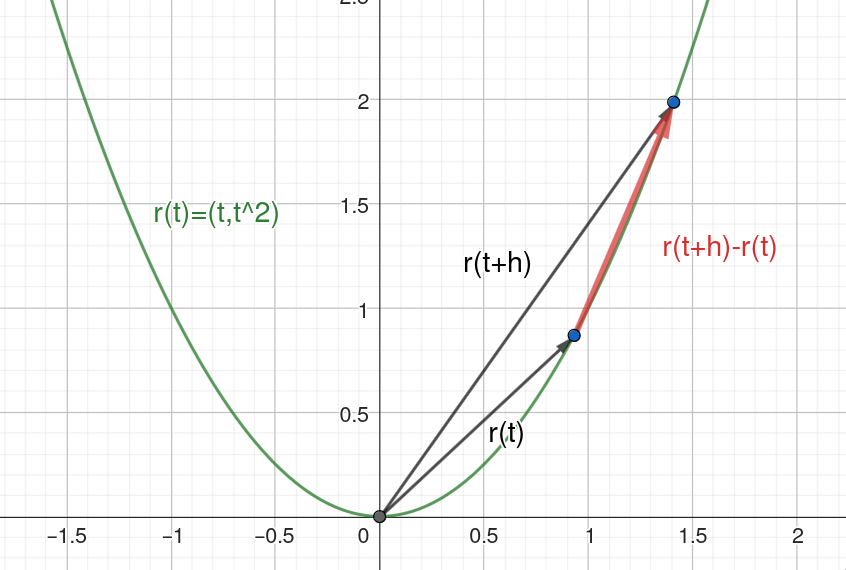
\includegraphics[width=0.5\textwidth]{ img/2024-05-05-15-17-31.png}
\end{center}
Vediamo che la differenza fra i valori di $ r $ e' rappresentata da un vettore $ r(t+h)-r(t) $, che puo' essere scomposto come la somma del cambiamento rispetto alle direzioni della base ortonormale di riferimento, in questo caso le direzioni delle assi:\\
\begin{center}
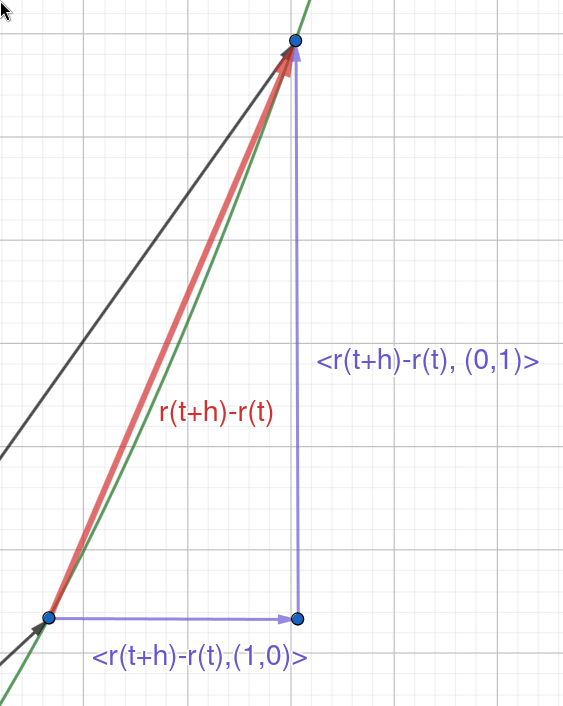
\includegraphics[width=0.25\textwidth]{img/2024-05-05-15-54-02.png}
\end{center}

Il valore del cambiamento lungo l'asse $ x $ e' dato dalla derivata di $ r_1(t) $, mentre il valore lungo l'asse $ y $ e' dato dalla derivata di $ r_2(t) $. Quindi possiamo applicare la definizione di limite e calcolare il rapporto incrementale in questo modo:
\[
  \lim_{h \to 0}\frac{r(t+h)-r(t)}{h} = \left(\lim_{h\to 0}\frac{r_1(t+h)-r_1(t)}{h}, \lim_{h \to 0}\frac{r_2(t+h)-r_2(t)}{h}\right) = (r_1'(t), r_2'(t))
\]
Ovvero, la derivata un punto $ t $ di una curva $ r:\mathbb{R}\to\mathbb{R}^n $ e' data dalla somma delle derivate delle $ n $ funzioni parametriche di $ r $ moltiplicate per il corrispondente vettore base $ e_k $. Quindi diamo la definizione:
\dfn{Velocita di una curva}{
  La velocita' (o derivata) di una curva e' il vettore tangente alla curva data:
  \[
    r'(t) = (r_1'(t),...,r_n'(t))
  \]
}
Quindi la direzione del vettore velocita' e' tangente alla curva nel punto dato, ma la sua lunghezza cosa indica?\\
Prendiamo due curve $ r(t) = (t, t^2),r' = (2t, 4t^2) $ e consideriamo il parametro $ t $ come il tempo trascorso. Notiamo che le due curve tracciate sono identiche, ma che una ci mette la meta' del tempo per percorrerla rispetto all'altra:
\begin{center}
  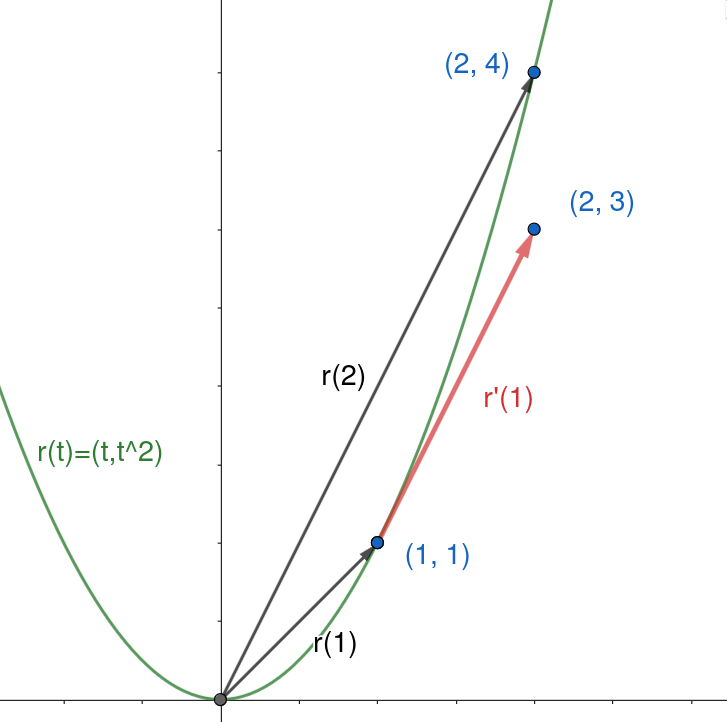
\includegraphics[width=0.2\textwidth]{img/2024-05-05-17-05-56.png}
  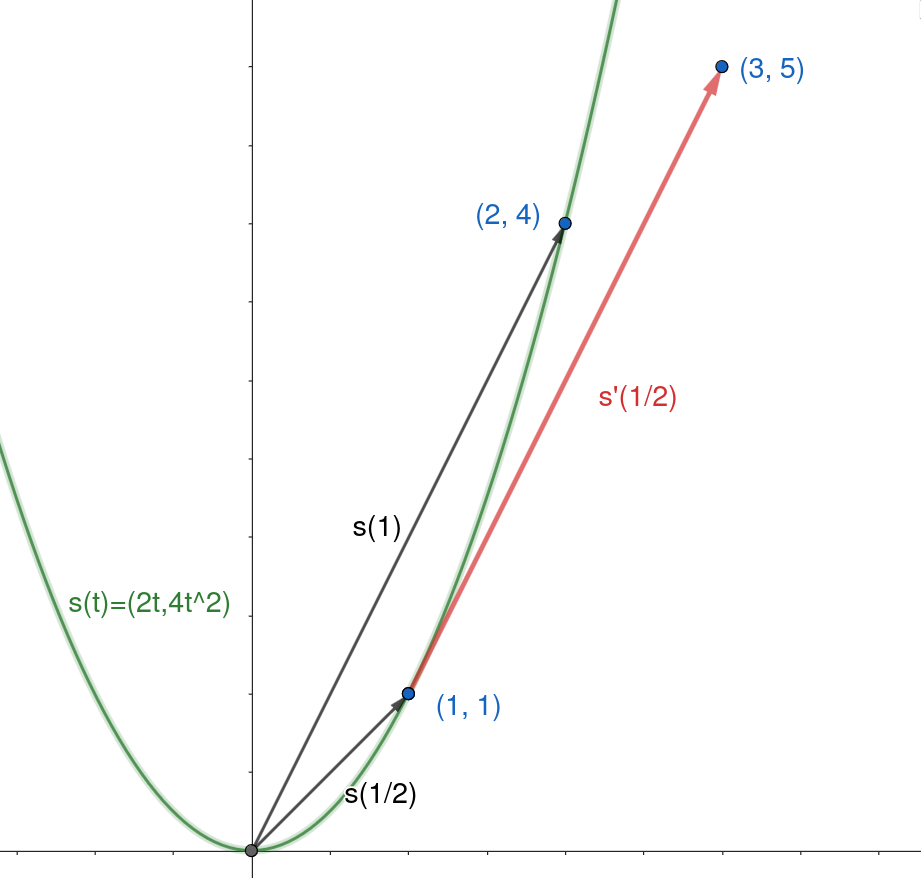
\includegraphics[width=0.2\textwidth]{img/2024-05-05-17-02-33.png}
\end{center}
Inoltre, la lunghezza del vettore velocita' nello stesso punto sulla curva e' doppia nella funzione piu' "veloce". Quindi possiamo intuire che la norma della derivata ci indica quanto "velocemente" ci stiamo muovendo nel punto dato della curva, chiamata anche \textbf{velocita' instantanea}:
\dfn{Velocita' scalare (instantanea)}{
  Non e' altro che la norma del vettore tangente, cioe':
  \[
    ||v(t)|| = ||r'(t)|| = \sqrt{(r_1'(t))^2+...+(r_n'(t))^2}
  \]
}
\subsection{Altre definizioni}
\dfn{Curva regolare}{
  Una curva e' detta \textbf{regolare} in $ t_0 \in (a,b) $ se:
  \[
    r'(t_0) \neq \underline{0}
  \]
}
\nt{
  Una curva regolare $ r:(a,b)\to\mathbb{R}^n $ e' anche detta essere una \textbf{immersione} di $ (a,b) $ in $ \mathbb{R}^n $.}
\dfn{Punto singolare}{
  Se $ t_0 \in (a,b) $ e' tale per cui
  \[
    r'(t_0) = \underline{0}
  \]
  Allora $ t_0 $ e' chiamato \textbf{punto singolare}
}
\dfn{Curve semplici}{
  Una curva e' detta \textbf{semplice} se e' iniettiva. (Cioe' la curva non si interseca)
}
\subsection{Curvatura}
Nelle curve almeno $ C^2 $, si definiscono:
\dfn{Curvatura}{
  Si definisce \textbf{curvatura} di $ r:(a,b)\to\mathbb{R}^n $ il modulo della accelerazione
  \[
    k = ||a(t)|| = ||v'(t)|| = |||r''(t)|
  \]
}
\dfn{Raggio di curvatura}{
  Si chiama \textbf{raggio di curvatura}
  \[
  R = \frac{1}{k}
  \]
  Bisogna considerarlo nella retta reale estesa $ \overline{\mathbb{R}} = [-\infty,+\infty] $, dato che le rette hanno il raggio di curvatura e ha senso che questo sia $ \infty $
}
\subsection{Derivata di una funzione scalare lungo una curva}
Prendiamo una funzione scalare $ f:\mathbb{R}^2\to\mathbb{R} $, definita come $ f(x,y) = x^2y $. Ora al posto delle due variabili di input $ x $ e $ y $ mettiamo due funzioni $ x(t)=cos(t) $ e $ y(t)=sin(t) $. Abbiamo ottenuto ora una funzione che dipende da un solo parametro $ (t) $, quindi e' possibile calcolare la sua derivata rispetto a questo parametro. Nel nostro esempio, possiamo espandere la nostra funzione in questo modo:
\[
  f(cos(t), sin(t)) = cos^2(t)sin(t)
\]
Quindi per calcolare la sua derivata basta applicare le classiche regole di derivazione:
\[
  \frac{d}{dt}f(cos(t), sin(t)) = -2cos(t)sin^2(t) + cos^3(t)
\]
Ma esiste un modo piu' generale per descrivere questo procedimento? Possiamo iniziare considerando una curva $ r:\mathbb{R}\to\mathbb{R}^2 $, che per seguire l'esempio sopra puo' essere definito come $ r(t) = (cos(t), sin(t)) $. Quindi ora possiamo usare il vettore dato dalla curva $ r $ come input alla nostra funzione scalare $ f $, creando quindi una composizione $ f \circ r: \mathbb{R}\to\mathbb{R} $ di cui vogliamo studiare la derivata. Analizziamo la situazione:
\begin{center}
  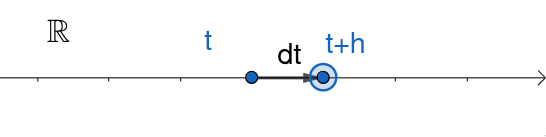
\includegraphics[width=0.5\textwidth]{img/2024-05-05-18-09-45.png}
\end{center}
\begin{center}
  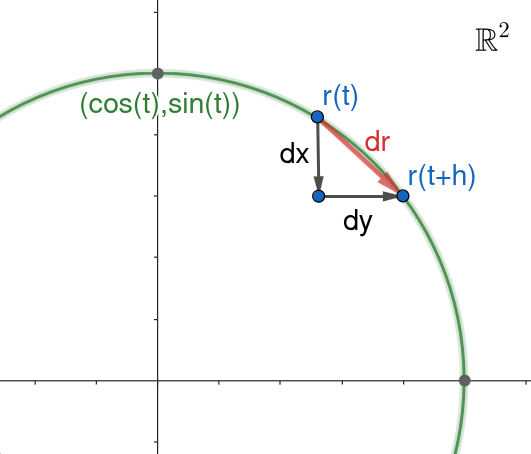
\includegraphics[width=0.5\textwidth]{img/2024-05-05-18-18-30.png}
\end{center}
\begin{center}
  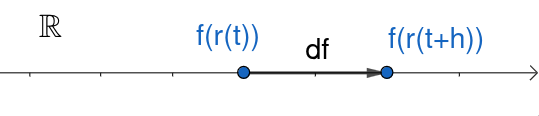
\includegraphics[width=0.5\textwidth]{img/2024-05-05-18-08-01.png}
\end{center}
Le tre figure ci mostrano, dall'alto verso il basso, come si propaga un aumento (infinitesimo) del parametro iniziale $ dt $, prima nella curva $ r $, poi dal valore spostato di $ r $ in $ f $. Alla fine otteniamo lo spostamento totale, chiamato $ df $ che ora vediamo come calcolare:
\begin{itemize}
  \item Prima di tutto, dobbiamo calcolare il valore del vettore $ r(t+h)-r(t) $, ovvero dobbiamo trovare lo "spostamento" causato da un aumento infinitesimo del parametro di input di $ r $. Se conosciamo la derivata della curva in quel punto, basta moltiplicarla per $ dt $ e otteniamo il vettore $ dr $:
    \[
      dr = r'(t)dt = (\frac{dx}{dt}dt, \frac{dy}{dt}dt)
    \]
  \item Ora che abbiamo il cambiamento in $ r $, dobbiamo vedere come calcolare il cambiamento che questo causa in $ f $. Puo' essere utile considerare le due componenti di $ dr $, in modo da avere il delta del primo e del secondo parametro di $ f $ separatamente. In modo analogo al primo passo moltiplichiamo le derivate parziali con gli spostamenti dei parametri corrispondenti, sommandoli per trovare $ df $:
    \[
    df = \frac{\partial f}{\partial x}\frac{dx}{dt}dt + \frac{\partial f}{\partial y}\frac{dy}{dt}dt
    \]
  \item Ci rimane soltanto dividere l'equazione per $ dt $ per trovare la derivata:
    \[
    \frac{df}{dt} = \frac{\partial f}{\partial x}\frac{dx}{dt}+\frac{\partial f}{\partial y}\frac{dy}{dt}
    \]
    Che puo' essere riscritta come un prodotto scalare:
    \[
      \frac{df}{dt} = \innerproduct{\nabla f(r(t))}{r'(t)}
    \]
\end{itemize}
\thm{}{
  Sia $ f:\mathbb{R}^n\to\mathbb{R} $ differenziabile, allora data una curva $ r:(a,b)\to\mathbb{R}^n $ (derivabile) si ha che:
  \[
    f \circ r:(a,b)\to\mathbb{R}
  \]
  E' derivabile, e la sua derivata e' la \textbf{derivata lungo la curva} $ r $, e si ha:
  \[
    (f \circ r)'(t)= <\nabla f(r(t)), r'(t)>
  \]
}
Prima di dare una dimostrazione formale di questo teorema, dobbiamo definire lo sviluppo di Taylor al primo ordine di una curva:
\dfn{}{
  Data $ r:]a,b[\to\mathbb{R}^n $ derivabile, sia $ k \in \{1,...,n\} $. Lo sviluppo di Taylor per $ r_k:]a,b[\to\mathbb{R} $ in $ t \in ]a,b[ $ e':
  \[
    r_k(t+s) = r_k(t) + r_k'(t)s + o_k(s)
  \]
  Quindi $ r(t+s) = r(t) + r'(t)s + o(s) $ (dove $ o(s) = (o_1(s),...,o_n(s)) $). 
}
\pf{Dimostrazione formale}{ 
  Usando la definizione di derivata, $ (f \circ r)'(t) = \lim_{s\to 0} \frac{f(r(t+s)) - f(r(t))}{s} $. Dato che $ f $ e' differenziabile, possiamo sostituire il numeratore con $ \innerproduct{f'(r(t))}{r(t+s)-r(t)} + o(|r(t+s)-r(t)|) $. Essendo derivabile, possiamo usare lo sviluppo di Taylor al primo ordine della curva $ r $ per sostituire $ r(t+s)-r(t) $ con $ r'(t)s + o(s) $. Usando la proprieta' distributiva e raccogliendo il fattore $ s $, il limite diventa $ \innerproduct{f(r(t))}{r'(t)} + \lim_{s\to 0}\frac{\innerproduct{f(r(t))}{o(s)}+o(|r'(t)s+o(s)|)}{s} $. Dividendo la frazione, nel primo addendo possiamo spostare il divisore all'interno del prodotto scalare che diventa $ \innerproduct{f(r(t))}{\frac{o(s)}{s}} $, che per definizione di o-piccolo diventa nullo. Per il secondo addendo, con $ s\to 0 $ abbiamo che $ o(|r'(t)s+o(s)|) = o(s) $, quindi sempre per definizione di o-piccolo anche il secondo addendo si annulla e il limite si azzera. 
}
\subsection{Ortogonalita' gradiente-insiemi di livello}
Possiamo utilizzare questo nuovo teorema per dimostrare la relazione di ortogonalita' fra il gradiente di una funzione calcolata in un punto e la curva di livello che passa per quel punto.\\
Come esempio, prendiamo una funzione $ f:\mathbb{R}^2\to\mathbb{R} $ e tracciamone delle curve di livello:
\begin{center}
  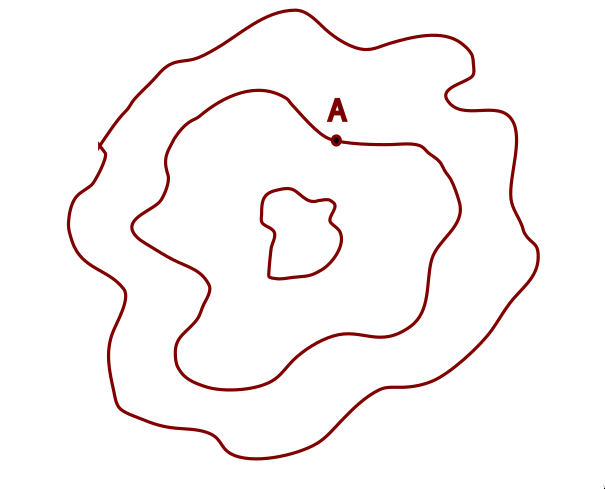
\includegraphics[width=0.5\textwidth]{img/2024-05-05-19-15-56.png}
\end{center}
Pensiamo ora di "zoomare" sul punto $ A $ e consideriamo la prossima curva di livello. Se ci avviciniamo abbastanza, possiamo considerare le due sezioni di curva come due linee parallele, quindi il segmento piu' corto che parte dal punto $ A $ e arriva alla prossima curva di livello e' quello perpendicolare alla curva di livello di $ A $:
\begin{center}
  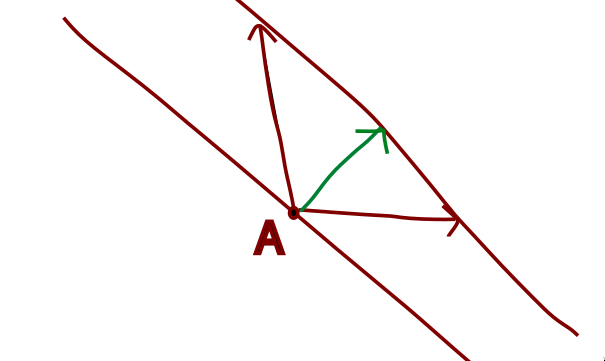
\includegraphics[width=0.5\textwidth]{img/2024-05-05-19-33-43.png}
\end{center}
Dato che la direzione perpendicolare alla curva di livello in $ A $ coincide con la direzione che ci porta piu' velocemente alla prossima curva di livello (direzione di massima crescita), possiamo intuire che il vettore gradiente in $ A $ e' perpendicolare alla curva che passa per $ A $:
\mprop{}{
  Data una funzione $ f:\mathbb{R}^n\to\mathbb{R} $ differenziabile, si ha che:
  \[
    \forall \underline{x} \in \mathbb{R}^n. \nabla f(\underline{x}) \perp L_{f(\underline{x})}
  \]
  Dove $ L_{f(\underline{x})} $ e' la curva di livello $ \{x \in \mathbb{R}^n|f(x)=f(\underline{x})\} $
}
\pf{Dimostrazione formale}{
  Assumiamo di avere una funzione $ f:\mathbb{R}^n\to\mathbb{R} $ differenziabile e un punto $ \overline{x} \in \mathbb{R}^n $. Supponiamo di poter costruire una curva $ r: ]-1,1[\to\mathbb{R}^n $ tale che: $ \forall t \in ]-1,1[. r(t) \in L_b $, $ r(0) = \overline{x} $ e $ r'(0) \in \mathbb{R}^n \neq \underline{0} $ (direzione tangente a $ L_{f(\overline{x})} $ nel punto $ \overline{x} $). Dato che tutti i punti della curva $ r $ fanno parte dello stesso insieme di livello, $ \forall t \in ]-1,1[. (f\circ r)(t) = f(\overline{x}) $. Essendo una funzione costante, sul suo dominio la derivata e' nulla, ovvero $ \forall t \in ]-1,1[. (f\circ r)'(t) = 0 $, che puo' essere scritta come $ \innerproduct{\nabla f(r(t))}{r'(t)} = 0 $ (usando il teorema di derivata lungo una curva). In altre parole, sappiamo che il prodotto scalare fra il gradiente di $ f $ in un punto e la derivata della curva di livello nello stesso punto e' sempre nullo. Quindi il gradiente in $ \overline{x} $ e' ortogonale alla tangente della curva di livello in $ \overline{x} $.
}
\chapter{Punti di massimo e minimo in piu' dimensioni}
La definizione di punti di massimo/minimo in piu' dimensioni e' molto simile a quella in $ \mathbb{R} $:
\dfn{Maxima e minima}{
  Data $ f:A\to\mathbb{R} $, con $ A \subseteq \mathbb{R} $, $ \underline{x} \in A $ si dice punto di massimo/minimo se:
  \[
    \exists \delta > 0. \forall x \in D(\underline{x},\delta) \cap A. f(x) \geq (\leq) f(\underline{x})
  \]
}
Come facciamo a trovare questi punti? Guardiamo i metodi usati in una dimensione per vedere se sono generalizzabili:
\begin{itemize}
  \item Studio del segno della derivata prima: se $ f(\underline{x}) = 0 $ e in un intorno di $ \underline{x} $ si ha che $ f(x) > (<) 0 $, allora $ \underline{x} $ e' un punto di massimo (minimo)
  \item Utilizziamo il segno della derivata seconda per trovare la concavita' del grafico nei punti di stazionamento:
    \[
    \begin{cases}
      f'(\underline{x}) = 0& \\
      f''(\underline{x}) > (<) 0 & 
    \end{cases} \iff \underline{x} \text{ e' punto di massimo (minimo)} 
    \]
\end{itemize}
Quando $ n \geq 2 $, $ f'(x) $ viene sostituito dal gradiente $ \nabla f(x) $, che e' un vettore e non uno scalare. Dato che non ha senso chiedersi se un vettore e' $ \geq 0 $,  il concetto di "crescente" e "decrescente" non puo' essere applicato in piu' dimensioni (perche' puo' essere diversa in direzioni diverse). Quindi dobbiamo utilizzare il secondo metodo, che ci da' due condizioni da rispettare (una sulla derivata di primo grado, una sulla seconda). Vediamo come generalizzare queste condizioni in piu' dimensioni:
\section{Condizioni del primo ordine}
Guardiamo la prima condizione relativa alla derivata di primo grado. Questa ci dice che e' condizione necessaria (ma non sufficente) per un punto di massimo/minimo avere la derivata prima nulla, vediamo se cio' vale anche in piu' dimensioni:
\thm{Fermat}{
  Data $ f:A\to\mathbb{R} $ differenziabile, con $ A \subseteq \mathbb{R}^n $ aperto, si ha che se un punto $ \underline{x} \in A $ e' massimo o minimo, allora:
  \[ 
    \nabla f(\underline{x}) = 0
  \]
}
\pf{Dimostrazione}{
  Presa una funzione $ f:A\to\mathbb{R} $ ($ A \subseteq \mathbb{R}^n $ aperto) con punto minimo in $ \overline{x} $, devo dimostrare che le derivate parziali in quel punto siano nulle. Semplicemente basta guardare la funzione sui piani paralleli alle direzioni canoniche passanti per $ \overline{x} $ e usare Fermat per le funzioni semplici. Per fare cio' creiamo una funzione $ h_k:]-\delta, \delta[\to\mathbb{R} $, definita $ \forall k \in \{1,...,n\} $ come $ h_k(t) = f(\overline{x} + te_k) $. Il $ \delta $ scelto e' quello garantito dalla definizione di punto minimo, quindi si ha che $ \forall x  $ che dista meno di $ \delta $ da $ \overline{x} $ si ha che $ f(x) \leq (\geq) f(\overline{x}) $. Quindi $ h $ ha max/min con $ t=0 $, ed essendo una funzione semplice abbiamo che $ h_k'(0) = 0 $. Ora dimostriamo che cio' implica che tutte le derivate parziali sono nulle: $ h_k'(0)=\lim_{t\to 0}\frac{h_k(t)+h_k(0)}{t} = \lim_{t\to 0}\frac{f(\overline{x}+te_k)+f(\overline{x})}{t} = \frac{\partial f}{\partial x_k}(\overline{x}) = 0 $.
}
Pero' questa e' solo una condizione necessaria, non sufficente per essere un punto di massimo/minimo. Vedremo infatti che esistono dei punti "di sella" che sono stazionari ma che non sono ne massimi ne minimi (sono una generalizzazione dei punti di flesso a tg orizzontale). Per distinguere i tipi di punti stazionari, dobbiamo guardare la derivata seconda:
\section{Condizioni di secondo ordine}
\subsection{In una variabile}
Diamo un attimo una intuizione al perche' la condizione di secondo ordine funziona in una variabile. Per fare cio', prendiamo una funzione $ f $ e scriviamone il polinomio di Taylor nel punto stazionario $ x_0 $ fino al secondo grado (dato che stiamo facendo solo un ragionamento informale, l'errore possiamo anche tralasciarlo):
\[
   f(x) \approx f(x_0) + f'(x_0)(x-x_0) + \frac{1}{2}f''(x_0)(x-x_0)^2 
\]
Dato che siamo interessati ai punti stazionari, $ f'(x_0) = 0 $, quindi possiamo semplificare l'approssimazione cosi':
\[
  f(x) \approx f(x_0) + \frac{1}{2}f''(x_0)(x-x_0)^2
\]
Dato che questa e' un'approssimazione di un piccolo intorno centrato nel punto $ x_0 $, se vediamo che $ x_0 $ e' un max/min nell'approssimazione, allora significa che nella funzione effettiva $ f $ esiste un intervallo contenente $ x_0 $ dove questo e' maggiore/minore di tutti i punti dell'intervallo. Guardiamo i vari casi:
\begin{itemize}
  \item Se $ f''(x_0) > 0 $, allora $ x_0 $ e' un punto di minimo, dato che $ (x-x_0)^2 $ e' sempre positivo tranne quando $ x = x_0 $, che ci darebbe il valore del minimo $ f(x_0) \approx f(x_0) + 0 $.
    \begin{center}
      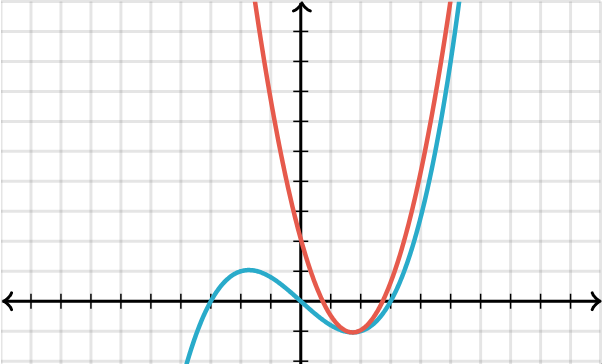
\includegraphics[width=0.5\textwidth]{img/2024-05-10-12-37-28.png}
    \end{center}
  \item Se $ f''(x_0) < 0 $, allora $ x_0 $ e' un punto di massimo, dato che siamo nella situazione precedente ma $ (x-x_0)^2 $ e' moltiplicato per una costante negativa. Quindi il polinomio descrive una parabola "all'ingiu'", con vertice in $ x_0 $.
    \begin{center}
      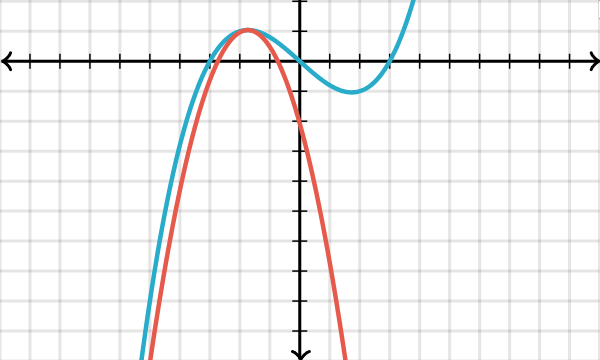
\includegraphics[width=0.5\textwidth]{img/2024-05-10-12-38-04.png}
    \end{center}
  \item Se $ f''(x_0) = 0 $, allora siamo in un caso particolare dove la derivata seconda non riesce a darci informazioni aggiuntive rispetto alla natura del punto stazionario.
  \begin{center}
    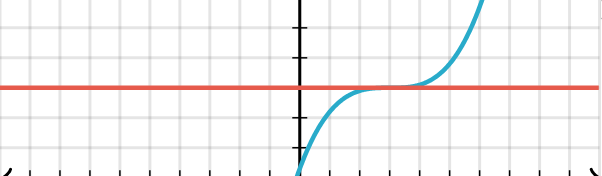
\includegraphics[width=0.5\textwidth]{img/2024-05-10-12-38-41.png}
  \end{center}
\end{itemize}
Quindi, per riassumere: quando $ f'(x_0) = 0 $, sappiamo che se il termine quadratico dell'approssimazione di Taylor $ \frac{1}{2}f''(x_0)(x-x_0)^2 $ e' sempre positivo/negativo (includendo lo 0), allora $ x_0 $ e' un punto di massimo/minimo.

\section{Approssimazione quadratica in piu' dimensioni}
Proviamo a seguire lo stesso procedimento per funzioni in una sola variabile. La prima cosa da fare e' scrivere un'approssimazione quadratica (Taylor al secondo ordine) di una funzione in piu' dimensioni. Partiamo prima con la definizione delle derivate seconde in n dimensioni:
\subsection{Derivate seconde e hessiana}
Introduciamo le derivate seconde in n dimensioni, ovvero il calcolo due volte di fila delle derivate (parziali). La differenza questa volta e' che ci sono diverse derivate parziali, che quindi possiamo applicare in sequenza in $ n^2 $ modi diversi. Introduciamo la notazione:
\dfn{Derivate seconde in n dimensioni}{
  Sia $ f:\mathbb{R}^n\to\mathbb{R} $, assumiamo che $ \forall k \in \{1,...,n\}. \exists \frac{\partial f}{\partial x_k} $ in ogni punto di $ \mathbb{R}^n $. Consideriamo una nuova variabile $ x_j $, con $ j \in \{1,...,n\} $, si ha che:
  \begin{itemize}
    \item Se $ j \neq k $ (ovvero se stiamo applicando due derivate parziali diverse) scriviamo:
      \[
        \frac{\partial }{\partial x_j}(\frac{\partial f}{\partial x_k}) = \frac{\partial^2 f}{\partial x_j \partial x_k}
      \]
    \item Nel caso $ j = k $ (applichiamo due volte la stessa derivata parziale) scriviamo:
      \[
        \frac{\partial }{\partial x_j}(\frac{\partial f}{\partial x_k}) = \frac{\partial^2 f}{\partial x_k^2}
      \]
  \end{itemize} 
}
Seppure sembrano tante, in verita' si puo' dimostrare che l'ordine in cui applichiamo le derivate non cambia il valore finale:
\thm{Schwarz}{
  Sia $ f:\mathbb{R}^n\to\mathbb{R} $ tale che per qualche (almeno uno) intorno centrato in $ p \in \mathbb{R}^n $ la derivata seconda (non mista!) di $ f $ e' continua, allora:
  \[
   \forall k,j \in \{1,...,n\}. \frac{\partial^2 f}{\partial x_k \partial x_j} = \frac{\partial^2 f}{\partial x_j \partial x_k}
  \]
}
Come abbiamo visto sopra, con $ n $ derivate parziali diverse esistono $ n^2 $ combinazioni di derivate seconde. Queste derivate seconde le possiamo mettere in una matrice (detta "hessiana") quadrata $ Hf(\overline{x}) \in M_n(\mathbb{R}) $ definita cosi':
\[
  Hf(\overline{x})_{jk} = \frac{\partial^2 f}{\partial x_j \partial x_k }
\]
\ex{}{
  Data una funzione in due dimensioni $ f:\mathbb{R}^2\to\mathbb{R} $, la sua matrice hessiana associata nel punto $ x_0 $ e':
  \[
    H_{f(x_0)} = \begin{pmatrix}
    \frac{\partial^2 f}{\partial x^2} & \frac{\partial^2 f}{\partial x \partial y} \\
    \frac{\partial^2 f}{\partial y \partial x} & \frac{\partial^2 f}{\partial y^2}\\
    \end{pmatrix}
  \]
  Ho omesso l'esplicitazione del punto da derivare nella matrice perche' spesso si fa cosi'.
}
\subsection{Taylor secondo Lagrange}
Torniamo un attimo in una dimensione per dare una nuova formula di approssimazione, che come noteremo da' informazioni aggiuntive rispetto a Taylor con il resto di Peano:
\thm{Taylor secondo Lagrange}{
  (n=1) $ f:\mathbb{R}\to\mathbb{R} $ assumo $ f,f',f'' $ continue. Dati $ \overline{x} $ e $ \overline{x} +h \in \mathbb{R} $, esiste $ \theta \in (0,1) $.
  \[
    f(\overline{x}+h) = f(\overline{x}) + f'(\overline{x})h + \frac{1}{2}f''(\overline{x}+\theta h)h^2
  \]
}
\nt{
  $ \overline{x} + \theta h $ appartiene all'intervallo di estremi $ \overline{x} $ e $ \overline{x} + h $ (aperto)
}
\nt{
  Ricordiamo la formula nota: $ f(\overline{x} + h) = f(\overline{x}) = f'(\overline{x})h+\frac{1}{2}f''(\overline{x})h^2 + o(h^2) $. Per $ h $ che non sono vicini a $ 0 $, la formula col resto di Peano non ci da molte informazioni riguardo all'errore, mentre con il resto di Lagrange abbiamo sempre una informazione quantitativa per qualunque $ h $ scelto.
}
\nt{
  Osserviamo che dalla formula di Lagrange possiamo ricondurci a quella sopra, quindi possiamo dire che contiene piu' "informazioni". Infatti sottraendo la seconda dalla prima rimane $ \frac{h^2}{2}(f''(\overline{x})-f''(\overline{x}+\theta h)) = o(h^2) $. Per verificarlo dividiamo la parte sinistra per $ h^2 $ e facciamo il limite per $ h \to 0 $, e si nota che effettivamente il limite e' $ 0 $ (usando la continuita' di $ f'' $). 
}
\subsection{Forma quadratica}
Per classificare i punti stazionari dobbiamo analizzare la parte quadratica dello sviluppo di Taylor, che come poi dimostreremo ha la seguente forma:
\[
ax^2 + 2bxy + cy^2
\]
Un'equazione di questo tipo e' chiamata una \textbf{forma quadratica}, che puo' essere rappresentata anche tramite il prodotto scalare fra una matrice e due vettori, che e' utile in quanto una sola scrittura vale per qualsiasi numero di variabili. Vediamo che in questo modo l'equazione diventa:
\[
  \innerproduct{\begin{pmatrix}
  a & b\\
  b & c\\
  \end{pmatrix}\begin{pmatrix}
  x\\
  y\\
  \end{pmatrix}}{\begin{pmatrix}
  x\\
  y\\
  \end{pmatrix}}
\]
Notiamo che la matrice associata alle forme quadratiche e' sempre una matrice simmetrica. Vediamo ora la definizione di forma quadratica usando questa nuova scrittura:

\dfn{Forma quadratica}{
  Sia $ A \in M_n(\mathbb{R}) $ simmetrica ($ A = A^T $) e $ h \in \mathbb{R}^n $ (vettore colonna $ n\times 1 $), definiamo la funzione $ q_A: \mathbb{R}^n\to\mathbb{R} $:
  \[
    q_A(h) = \innerproduct{Ah}{h} \in \mathbb{R} 
  \] 
}
\nt{
  $ p(h) = 3h_1^2 + \frac{1}{3}h_1h_2 - 7h_2^2 $, quindi $ p = q_A $ con $ A = \begin{pmatrix}
  3 & 1/6\\
  1/6 & -7\\
  \end{pmatrix} $
}
\subsubsection{Segno}
Per generalizzare la condizione $ f''(\overline{x})> 0 $ in $ \mathbb{R} $ dobbiamo dare una nozione di segno di una forma quadratica:
\dfn{}{
  Sia $ A = A^T \in M_n(\mathbb{R}) $. Allora si dice che:
  \begin{itemize}
  \item $ A $ e' definita positiva se $ \innerproduct{Ah}{h} > 0 $ $ \forall h \neq 0 $
  \item $ A  $ e' definita negativa se $ \innerproduct{Ah}{h} < 0 $ $ \forall h \neq 0 $
  \item $ A $ e' indefinita se $ \exists h, t \in \mathbb{R}^n. \innerproduct{Ah}{h} < 0 < \innerproduct{At}{t} $
  \end{itemize}
}
\nt{
  Tutte le disuguaglianze sono strette
}
Per ora restringiamoci a solo due variabili. E' possibile sapere il segno di una forma quadratica conoscendo solo la sua matrice? Si, si puo' dimostrare trattando inizialmente $ y $ come una costante, chiamiamola $ y_0 $, e calcolando gli zeri:
\[
  y_0\left(\frac{-b \pm \sqrt{b^2-ac}}{a}\right)
\]
Vediamo subito che se $ y_0 = 0 $, allora abbiamo entrambe gli zeri nel punto $ (0,0) $, mentre se $ y_0 \neq 0 $ il numero di zeri dipende dal delta (in realta' studiamo il meno-delta per poter usare il determinante dopo). La concavita' della parabola, invece, dipende come al solito dal segno di $ a $:
\begin{itemize}
  \item se $ ac-b^2 < 0 $, allora esistono due zeri distinti $ \forall y_0 \neq 0 $ e la parabola e' sia negativa che positiva, quindi in questo caso la forma quadratica e' indefinita.
  \item se $ ac-b^2 > 0 $, non esistono zeri reali e quindi la parabola e' tutta positiva se $ a>0 $ o tutta negativa se $ a < 0 $. Quindi il segno della forma quadratica dipende dal segno di $ a $.
  \item se $ ac-b^2 = 0 $, allora esistono punti $ (x,y) \neq (0,0) $ per cui il valore della forma quadratica e' $ 0 $ e il resto dell'immagine e' tutta positiva o tutta negativa. Per questo motivo non riusciamo a dire che sia sempre positiva o negativa, ne che sia indefinita.

\end{itemize}
Il valore $ ac-b^2 $ in realta' corrisponde al determinante della matrice associata alla forma quadratica, quindi possiamo riscrivere i casi sopra in modo piu' breve:
\mprop{Regola dei segni delle forme quadratiche}{
  Sia $ A = \begin{pmatrix}
  a & b\\
  b & c\\
  \end{pmatrix} $. Allora:
  \begin{itemize}
  \item $ A > 0 \iff \begin{cases}
  a > 0 & \\
  detA > 0 & 
  \end{cases} $
    \item $ A < 0 \iff \begin{cases}
    a < 0 & \\
    detA > 0 & 
    \end{cases} $
    \item $ A $ e' indefinita $ \iff $ $ detA < 0 $ (punto di sella)
  \end{itemize}
}

\subsubsection{Forma quadratica Hessiana}
Essendo una matrice simmetrica, anche la matrice hessiana, che abbiamo definito insieme alle derivate seconde in $ n $ dimensioni, ha una forma quadratica associata:
\[
  q(h) = \innerproduct{H_{f(\overline{x})}h}{h}
\]
dove $ H_{f(\overline{x})} $ e la matrice hessiana di ordine $ n $ e $ h $ e' un qualunque vettore di $ \mathbb{R}^n $.

\subsection{Taylor di secondo ordine in n dimensioni}
\thm{Formula di Taylor con resto di Lagrange di secondo ordine in n dimensioni}{
  Data una funzione $ f:\mathbb{R}^n\to\mathbb{R} $ con tutte le derivate seconde continue, si ha che $ \forall x_0, h \in \mathbb{R}^n $, $ \exists \delta \in (0,1) $ tale che:
  \[
    f(x_0 + h) = f(x_0) + \innerproduct{\nabla f(x_0)}{h} + \frac{1}{2} \innerproduct{H_{f(x_0 + \delta h)}h}{h}
  \]  
}
\nt{
  Come avevamo visto in una dimensione, questa formula e' "globale", ovvero vale anche per $ h $ "lontani" da $ x_0 $.
}
\pf{}{
  Usiamo una funzione $ h: \mathbb{R}\to\mathbb{R} $ che ha derivata seconda continua (?). Per Taylor in una variabile sappiamo che: $ \forall t_0, t_0+t \in \mathbb{R}. \exists \theta \in ]0,1[: h(t_0+t) = h(t_0) + h'(t_0)t + \frac{1}{2}h''(t_0+\theta t)t^2 $. Prendendo come $ f $ la funzione del teorema e dati $ x_0, x_0+h \in \mathbb{R}^n $, definisco la funzione $ h(t) = f(x_0+th) $ (stare attenti a non confondere $ h $-funzione con $ h $-variabile). Scriviamo Taylor di $ h $ ponendo $ t_0 = 0 $ e $ t = 1 $: $ h(1) = h(0) + h'(0) + \frac{1}{2}h''(\theta) $. Usando la definizione di $ h(t) $, otteniamo $ h(1) = f(x_0 + h) $, $ h(0) = f(x_0) $, $ h'(0) = \innerproduct{\nabla f(x_0)}{h} $ (derivata di f lungo la curva $ v(t) = x_0+th $) e $ h''(\theta) = \innerproduct{H_{f(x_0+\theta h)h}}{h} $. Sostituendo otteniamo la tesi del teorema. 
}
\cor{Taylor di secondo ordine in n dimensioni con resto di Peano}{
  Data una funzione $ f:\mathbb{R}^n\to\mathbb{R} $ con tutte le derivate seconde continue, si ha che $ \forall x_0,h \in \mathbb{R}^n $ si ha che:
  \[
    f(x_0 + h) = f(x_0) + \innerproduct{\nabla f(x_0)}{h} + \frac{1}{2} \innerproduct{H_{f(x_0)}h}{h} + o(\norm{h}^2)
  \]
  Dove $ \forall \epsilon > 0. \exists \delta > 0. \forall 0 < \norm{h} < \delta \implies \left|\frac{o(\norm{h}^2)}{\norm{h}^2}\right| < \epsilon $
}
\pf{}{
  Scriviamo Taylor nelle due versioni:
  \[
    f(x_0+h) = f(x_0) + \innerproduct{\nabla f(x_0)}{h} + \frac{1}{2} \innerproduct{H_{f(x_0 + \theta h)}h}{h}
  \]
  \[
    f(x_0+h) = f(x_0) + \innerproduct{\nabla f(x_0)}{h} + \frac{1}{2} \innerproduct{H_{f(x_0)}h}{h} + o(|h|^2)
  \]
  Sostituiamo il membro a sinistra del secondo con il membro di destra del primo, e semplificando otteniamo:
  \[
    \frac{1}{2} \innerproduct{H_{f(x_0 + \theta h)}h}{h} - \frac{1}{2}\innerproduct{H_{f(x_0)}h}{h} = o(|h|^2)
  \]
  Moltiplichiamo per 2 e scriviamo le forme quadratiche per esteso raccogliendo i termini con le stesse derivate seconde. Otteniamo una somma di tre forme di questo tipo (dove $ j,k \in \{1,...,n\} $):
  \[
    h_jh_k(\partial_{jk}f(x_0+\theta h)-\partial_{jk}f(x_0))
  \]
  Dobbiamo mostrare che questa somma sia un o-piccolo di $ |h|^2 $, quindi basta controllare che $ \forall j,k \in \{,...,n\} $:
  \[
    \lim_{h\to(0,0)} \frac{h_jh_k}{|h|^2}(\partial_{jk}f(x_0+\theta h)-\partial f(x_0)) = 0
  \]
  Per analisi asintotica, $ \frac{h_jh_k}{|h|^2} $ tende a un numero reale, mentre il fattore a destra tende a 0.
}

\section{Classificazione di punti stazionari}
Diamo prima di tutto una definizione formale di punto di sella:
\dfn{Punto di sella}{
  Data una funzione $ f:\mathbb{R}^n\to\mathbb{R} $ con derivate seconde continue, il punto critico $ \overline{x} \in \mathbb{R}^n $ ($ \nabla f(\overline{x}) = \underline{0} $) si dice di \textbf{sella} se:
  \[
    \forall \delta > 0. \exists \overline{x}^-,\overline{x}^+.f(\overline{x}^-) < f(\overline{x}) < f(\overline{x}^+)
  \]
}
Ci serve anche una proprieta' delle forme quadratiche:
\mprop{}{ \label{valoreMinimo}
  Sia $ A = A^T $ definita positiva di ordine $ n $, allora $ \exists \lambda \in \mathbb{R} > 0 $ tale che $ \forall h \in \mathbb{R}^n $:
  \[
  \innerproduct{Ah}{h} \geq \lambda \norm{h}
  \]
  Possiamo anche scrivere $ \innerproduct{A\frac{h}{\norm{h}}}{\frac{h}{\norm{h}}} \geq \lambda $.
}
\pf{Dimostrazione in $ \mathbb{R}^2 $}{
  Prendiamo una matrice simmetrica di ordine 2 $ A $ definita positiva, con $ a,b,c \in \mathbb{R} $. Dobbiamo dimostrare che esiste un $ \lambda \in \mathbb{R} > 0 $ tale che per ogni vettore unitario $ v = (cos\theta, sin\theta) $ si ha che $ \innerproduct{Av}{v} \geq \lambda $. Chiamiamo $ g: [0,2\pi]\to\mathbb{R} $ la forma quadratica ottenuta. Essendo $ g $ continua su un intervallo chiuso possiamo applicare Weierstrass e dire che esiste un minimo assoluto, ovvero $ \exists \overline{\theta} \in [0,2\pi].\forall \theta \in [0,2\pi]: g(\theta) \geq g(\overline{\theta}) $. Inoltre, dato che $ g $ e' definita positiva, $ \forall \theta \in [0,2\pi]. g(\theta) > 0 $, quindi $ g(\overline{\theta}) $ e' strettamente positiva ed equivale al valore $ \lambda $ cercato.
}
\nt{
  $ \lambda $ puo' essere scelto come l'autovalore minore di $ A $.
}
Ora siamo in grado di dimostrare come il segno della matrice hessiana puo' classificare un punto critico:
\thm{Classificazione dei punti critici}{
  Data una funzione $ f:\mathbb{R}^n\to\mathbb{R} $ con derivate seconde continue, sia $ \overline{x} \in \mathbb{R}^n $ un punto critico, allora:
  \begin{itemize}
    \item Se $ H_{f(\overline{x})} > 0 $, allora $ \overline{x} $ e' un punto di minimo
    \item Se $ H_{f(\overline{x})} < 0 $, allora $ \overline{x} $ e' un punto di massimo
    \item Se $ H_{f(\overline{x})}  $ e' indefinita, allora $ \overline{x} $ e' un punto di sella  
  \end{itemize}
}
\pf{}{
  \begin{itemize}
    \item $ 1) $ Per ipotesi sappiamo che $ \nabla f(\overline{x}) = 0 $ e che $ H_{f(\overline{x})} > 0 $. Dobbiamo dimostrare che $ \exists \delta \in \mathbb{R} > 0. \forall h \in \mathbb{R}^n.\norm{h} < \delta: f(\overline{x}+h) - f(\overline{x}) \geq 0 $ (definizione di minimo). Dato che $ f $ ha derivate seconde continue per ipotesi, possiamo scrivere il suo sviluppo di Taylor di secondo ordine: $ f(\overline{x}+h)-f(\overline{x}) = \frac{1}{2}\innerproduct{H_{f(\overline{x})}h}{h} + o(\norm{h}^2) $ (dato che il gradiente e' nullo). Per \ref{valoreMinimo} sappiamo che $ \innerproduct{H_{f(\overline{x})}h}{h} \geq \lambda \norm{h} $, quindi possiamo continuare l'equazione sopra aggiungendo $ \geq \frac{1}{2}\lambda \norm{h}^2 + o(\norm{h}^2) = \norm{h}^2 \left(\lambda+\frac{o(\norm{h}^2)}{\norm{h}^2}\right) $. Usiamo la definizione di o-piccolo, scegliendo come $ \epsilon $ il valore $ \frac{\lambda}{2} $ e attribuiamo al $ \delta $ che stiamo cercando il valore positivo per cui $ \forall h \in \mathbb{R}^n.\norm{h} < \delta: \left|\frac{o(\norm{h^2})}{\norm{h}^2}\right| < \frac{\lambda}{2} $. Controlliamo che $ \forall h . \norm{h} < \delta $ valga la proprieta' di minimo: $ \geq \frac{\norm{h}^2}{2}\left(\lambda - \frac{\lambda}{2}\right) \geq 0 $.
    \item $ 2) $ (Uguale a quello sopra)
    \item $ 3) $ 
  \end{itemize}
}


\chapter{Integrali su piu' variabili}
Vediamo ora come generalizzare il concetto di integrale definito in due dimensioni. Considero $ f: A\to\mathbb{R} $, $ A \subseteq \mathbb{R}^2 $, $ \forall (x,y) \in A. f(x,y) \geq 0 $, il nostro scopo e' quello di trovare il volume del sottografico rispetto all'area $ A $, ovvero dell'insieme di punti $ \{(x,y,z) \in \mathbb{R}^3 | (x,y) \in A, 0 \leq z \leq f(x,y)\} $.
\begin{center}
  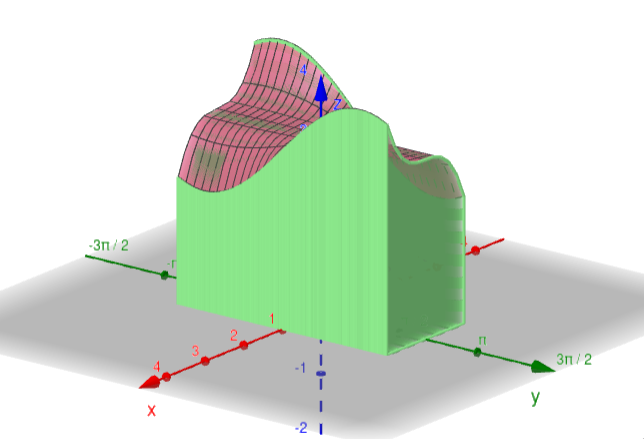
\includegraphics[width=0.5\textwidth]{img/2024-05-13-14-46-04.png}
\end{center}
Si dimostra che, se $ A $ e' \textbf{opportuno} ed $ f $ e' continua, il colume del sottografico e' dato da:
\[
  \int_{A}^{} f(x,y)dxdy = \text{ integrale doppio}
\]
Se mettiamo $ f = 1 $ costante, si trova $ \int_{A}^{} 1dxdy $ che ha lo stesso valore dell' area di A (come $ \int_{a}^{b}1dx = b-a $ = lunghezza di $ [a,b] $).
\section{Insiemi semplici}
\dfn{Insieme y-semplice nel piano $ xy $}{
  Sia $ [a,b] \subseteq \mathbb{R} $, siano $ g_1,g_2:[a,b]\to\mathbb{R} $, tali che $ g_1(x) \leq g_2(x) \forall x \in [a,b] $ (con $ g_1,g_2 $ continue). 
  \[
    A = \{(x,y) \in \mathbb{R}^2 | x \in [a,b], g_1(x) \leq y \leq g_2(x)\}
  \]
}
Si chiama y-semplice perche' intersecandolo con una retta verticale otteniamo sempre un segmento continuo:
\begin{center}
  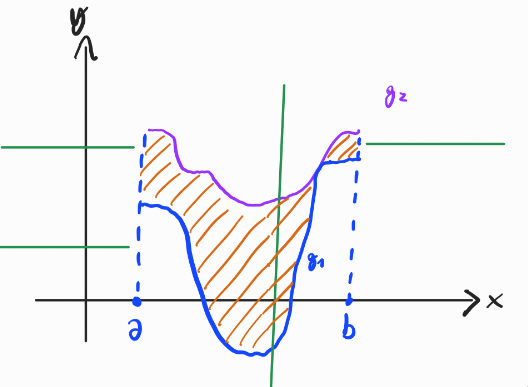
\includegraphics[width=0.35\textwidth]{img/2024-05-15-10-01-35.png}
\end{center}
Se abbiamo la stessa proprieta' ma per le rette orizzontali, allora sono insiemi x-semplici:
\dfn{Insieme x-semplice nel piano xy}{
  Sia $ [c,d] \subseteq \mathbb{R}_y $, siano $ h_1,h_2:[c,d]\to\mathbb{R} $, tali che $ h_1(y) \leq h_2(y) \forall y \in [c,d] $ (con $ h_1,h_2 $ continue). 
  \[
    A = \{(x,y) \in \mathbb{R}^2 | y \in [c,d], h_1(y) \leq x \leq h_2(y)\}
  \]
}
\begin{center}
  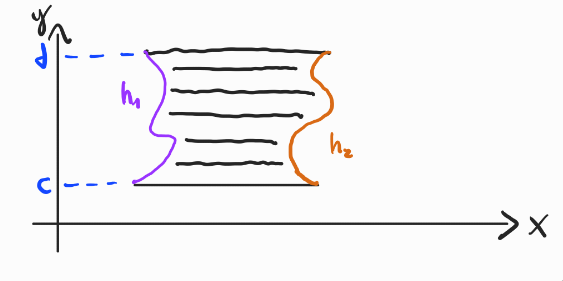
\includegraphics[width=0.35\textwidth]{img/2024-05-15-10-02-41.png}
\end{center}
\nt{
  Esistono insiemi che non sono ne' x, ne' y -semplici (corona circolare):
  \begin{center}
    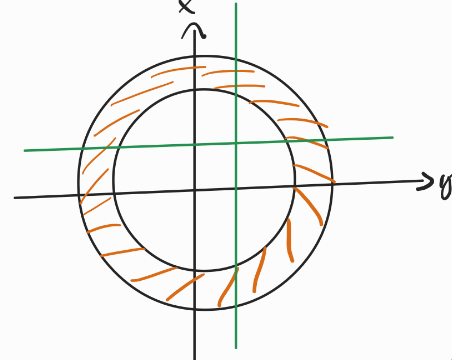
\includegraphics[width=0.25\textwidth]{img/2024-05-15-10-03-29.png}
  \end{center}
}

\section{Formule di riduzione}
Vediamo ora come le proprieta' degli insiemi semplici possano aiutarci a calcolare il volume di un sottografo in tre dimensioni. L'obbiettivo principale e' quello di calcolare l'area sotto il grafico fissando la $ x $ o la $ y $ usando un integrale in una variabile, e poi di sommare tutte queste aree lungo la direzione opposta utilizzando ancora un integrale semplice. Vediamo come applicare questa intuizione formalmente:
\mprop{Riduzione y-semplice}{
  Siano $ g_1,g_2:[a,b]\to\mathbb{R} $ due funzioni continue t.c. $ \forall x \in [a,b]. g_1(x) \leq g_2(x) $. Sia $ A \in \mathbb{R}^2 $ un insieme y-semplice e sia $ f:A\to\mathbb{R} $ continua, allora vale:
  \[
    \int_{A}^{}f(x,y)dxdy = \int_{a}^{b}\left(\int_{g_1(x)}^{g_2(x)}f(x,y)dy\right)dx
  \]
}
Quindi, dato un insieme $ A $ y-semplice e una funzione $ f:A\to\mathbb{R} $ continua, per trovare il volume del sottografo relativo ad $ A $ bisogna prima di tutto trovare la formula che ci da' l'area sotto il grafico dato un valore di $ x $. Quindi consideriamo la $ x $ come costante e applichiamo l'integrale in $ dy $:
\begin{center}
  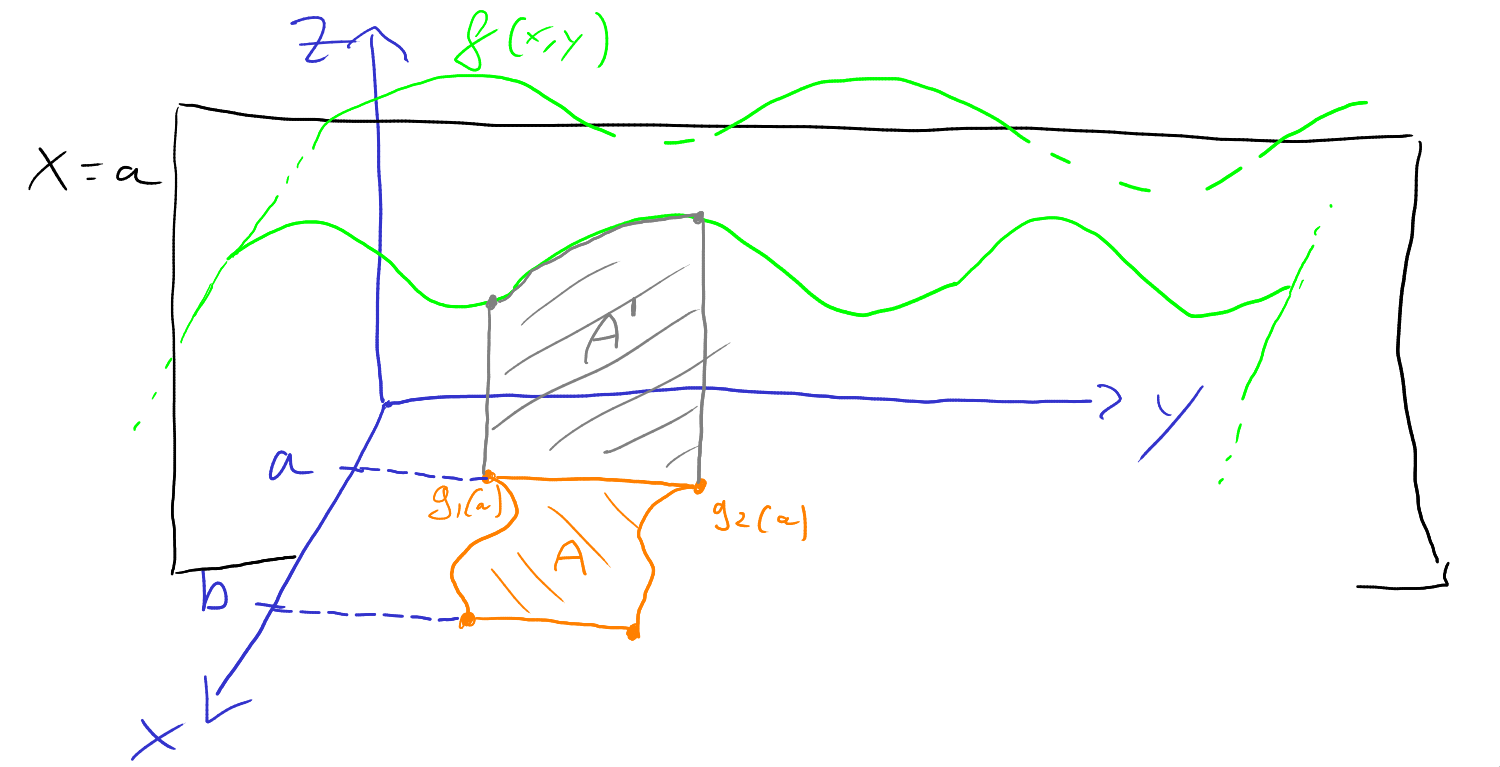
\includegraphics[width=0.5\textwidth]{img/2024-05-15-11-29-57.png}
\end{center}
Da notare come questi integrali sono calcolati sull'intervallo $ [g_1(x), g_2(x)] $, che sono sempre gli estremi dell'area dato che $ A $ e' y-semplice. Ora ci basta sommare tutte le aree trovate per tutti gli $ x $ nell'intervallo $ [a,b] $, che possiamo fare con un secondo integrale in $ dx $ questa volta:
\begin{center}
  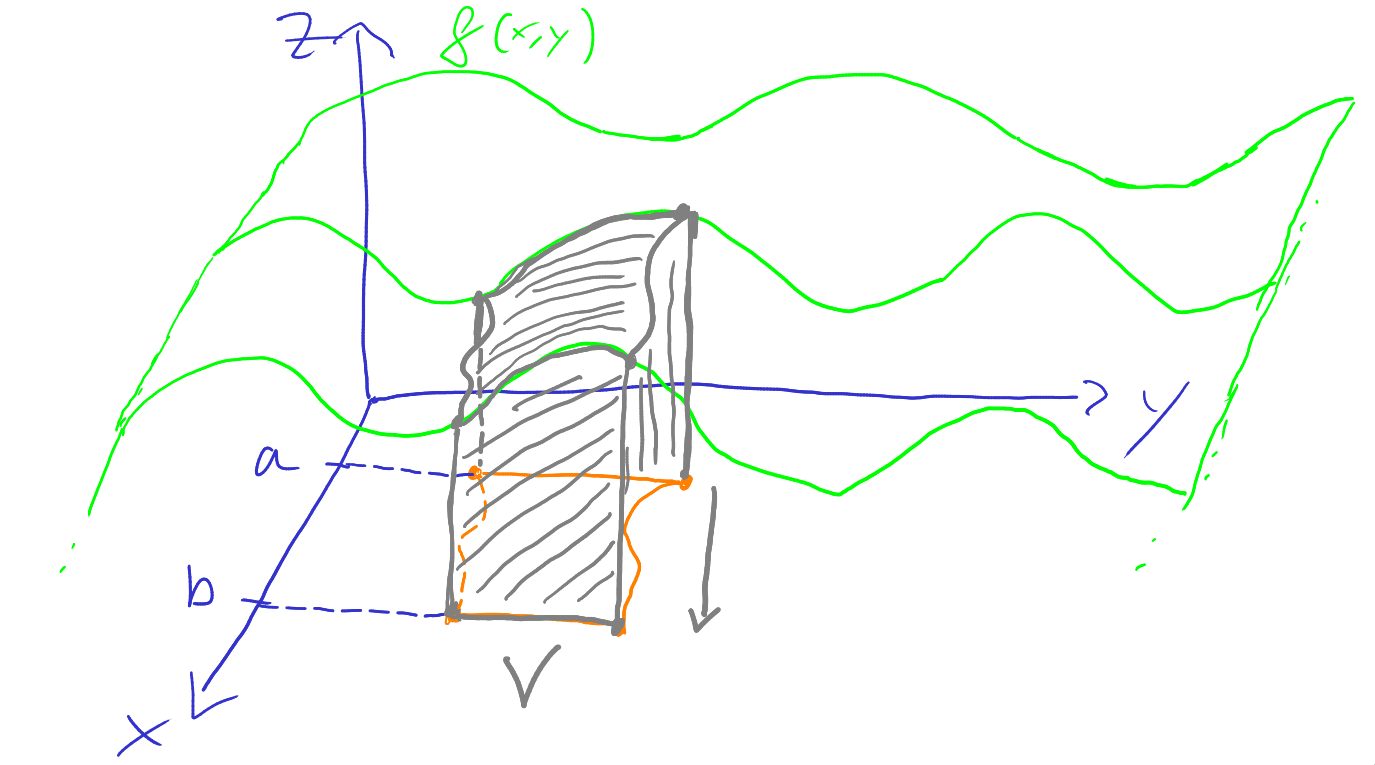
\includegraphics[width=0.5\textwidth]{img/2024-05-15-11-45-00.png}
\end{center}
Se dobbiamo calcolare il volume sopra un'area x-semplice, basta ripetere gli stessi passi trovando prima le aree fissando $ y $ e poi sommarle tutte lungo l'asse $ y $:
\mprop{Riduzione x-semplice}{
  Siano $ h_1,h_2:[c,d]\to\mathbb{R} $ due funzioni continue t.c. $ \forall y \in [c,d]. h_1(y) \leq h_2(y) $. Sia $ A \in \mathbb{R}^2 $ un insieme x-semplice e sia $ f:A\to\mathbb{R} $ continua, allora vale:
  \[
    \int_{A}^{}f(x,y)dxdy = \int_{c}^{b}\left(\int_{h_1(y)}^{h_2(y)}f(x,y)dx\right)dy
  \]
}


\end{document} 
